\documentclass[10pt,a4paper]{article}
\usepackage[utf8]{inputenc}
\usepackage[english,russian]{babel}
\usepackage{cmap}
\usepackage[OT1]{fontenc}
\usepackage{amsmath}
\usepackage{amsfonts}
\usepackage{amssymb}
\usepackage{graphicx}
\usepackage{float}
\usepackage{wrapfig}
\usepackage{caption}
\DeclareCaptionLabelSeparator{dot}{. }
\captionsetup{justification=centering,labelsep=dot}
\graphicspath{{pictures/}}
\DeclareGraphicsExtensions{.pdf,.png,.jpg,.eps}
\begin{document}

\part{Основы}


\textbf{6 Восприятие робота}\\

\textbf{6.1 Введение}\\

Модели измерения окружающей среды вместе с моделями движения составляют две, специфические для вероятностной робототехники, группы. Моделями измерений описывается процесс взаимодействия, посредством которого в физическом мире генерируются измерения датчиков. Сегодня в роботах используются самые разнообразные датчики, такие как датчики касания, измерения расстояния или видеокамеры. Специфика модели зависит от конкретного вида датчика: датчики изображения лучше всего моделируются с помощью проективной геометрии, а сонары – описанием звуковой волны и ее отражения от различных поверхностей в окружающей среде. 

В вероятностной робототехнике  обязательно моделируется шум датчиков, чтобы учесть изначальная неопределённость, присущую самому процессу измерения. Формально, модель измерений определяется в виде распределения условной вероятности $p(z_t | x_t, m)$, где $x_t$ – положение робота, $z_t$ – измерение в момент времени $t$, а $m$ – карта окружающей среды. Хотя в материале данной главы, в основном, описаны датчики расстояния, предлагаемые принципы и уравнения применимы и для других типов датчиков, таких, как видеокамера или детектор ориентиров на основе считывателя бар-кодов. 

СКАНИРОВАНИЕ ДАЛЬНОСТИ СОНАРОМ

Чтобы проиллюстрировать основную проблему мобильных роботов, использующих датчики для восприятия окружающей среды, на Рис. 6.1a показано типичное \textit{сканирование дальности сонаром}, в коридоре с помощью мобильного робота, оборудованного круговым массивом из 24 ультразвуковых датчиков. Значения расстояний, измеренные отдельными датчиками, выделены светло-серым цветом, карта окружающей среды показана чёрным. 
Большинство измерений соответствуют расстоянию до ближайшего объекта в конусе измерения. При этом на некоторых измерениях  отсутствуют обнаруженные объекты. 

\begin{figure}[H]
	\center{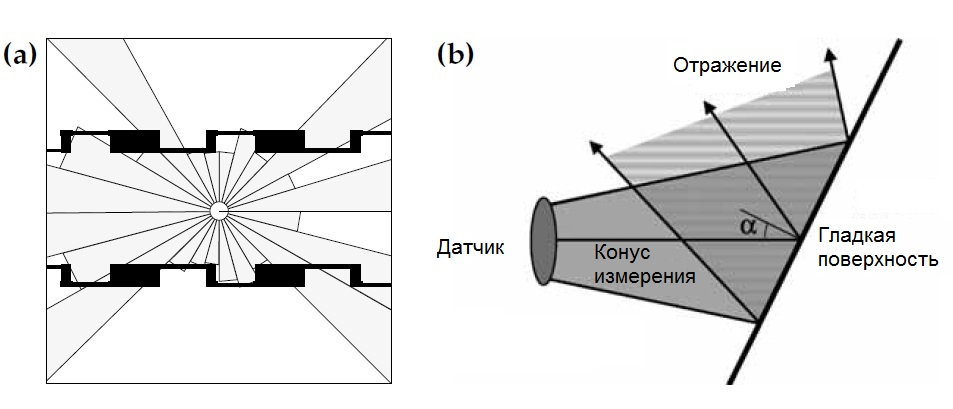
\includegraphics[width=1\linewidth]{61orig}}
	\caption{ (Рис. 6.1 (a) Типичное ультразвуковое сканирование роботом окружающей среды. (b) Ошибочное измерение ультразвукового измерения дальности. Такой эффект возникает при попадании сигнала сонара на отражающую поверхность под углом $\alpha$, превышающим половину угла раскрытия датчика.)}
	\label{fig:61orig}
\end{figure}

Неспособность датчиков надёжно измерить расстояние до близлежащих предметов часто называют шумами датчика.\\
ЗЕРКАЛЬНОЕ ОТРАЖЕНИЕ\\ 
Технически, такие шумы довольно предсказуемы, поскольку гладкие поверхности (например, стены), отражают звук зеркально, и можно считать, что стена для звуковой волны сонара является аналогом зеркала. Трудности возникают, в основном, когда звуковая волна сталкивается с гладкой поверхностью под углом. В таком случае эхо может распространяться в направлении, отличном от обратного, что показано на Рис. 6.1b. Этот эффект часто ведёт к слишком большим показаниям измерения, по сравнению с реальным расстоянием до ближайшего объекта в основном конусе. Вероятность возникновения такого эффекта зависит от ряда характеристик, например, материала поверхности, угла между нормалью к поверхности и направлением конуса датчика, расстояния до поверхности, ширины основного конуса датчика, чувствительности сонара. Другие ошибки, такие как слишком малые показания, могут вызываться перекрёстными наводками между разными датчиками (звук распространяется медленно!) или присутствием не смоделированных объектов, например, людей, в непосредственной близости от робота. 

СКАНИРОВАНИЕ РАССТОЯНИЯ ЛАЗЕРОМ
 
На Рис. 6.2 показано типичное \textit{сканирование расстояния лазером}, полученное с помощью 2D лазерного дальномера. Лазер аналогичен сонару в том смысле, что он тоже активно излучает сигнал и записывает эхо, но в случае лазера сигнал – это световой луч. Ключевая разница с сонаром состоит в том, что лазеры позволяют получить гораздо более сфокусированные лучи. Лазер, изображённый на Рис. 6.2, измеряет расстояние по величине запаздывания отражённого сигнала, при этом измерения разделены углом в один градус. 

Как правило, чем точнее модель датчика, тем лучше результаты измерений, хотя некоторые важные замечания по этому поводу уже обсуждались в подразделе 2.4.4. На практике довольно часто  точное моделирование датчика невозможно, в основном, в силу сложности происходящих в них физических процессов.

\begin{figure}[H]
	\center{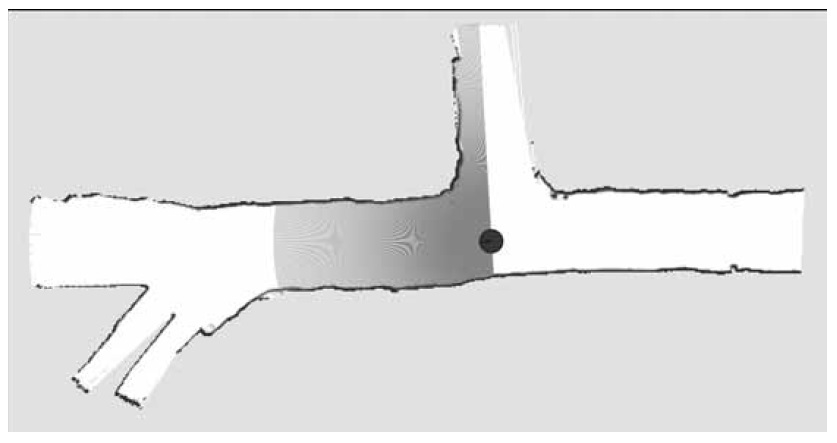
\includegraphics[width=1\linewidth]{62orig}}
	\caption{ (  Рис. 6.2 Типичное сканирование расстояния лазерным лучом, полученное с лазера SICK LMS. Окружающая среда, показанная на рисунке – угольная шахта. Изображение принадлежит Дирку Хёнелу (Dirk Hähnel), университет Фрайбурга.)}
	\label{fig:62orig}
\end{figure}

Часто характеристики отклика датчика зависят от переменных, которые не хотелось бы явно описывать в вероятностном алгоритме робота (например, материал поверхности стен, который, без особой необходимости, не указывается при составлении карт для робота). Вероятностная робототехника обрабатывает стохастические неточности моделей датчиков путём моделирования процесса измерения в виде плотности условной вероятности $p(z_t | x_t)$, а не детерминированной функции $z_t = f(x_t)$. В силу этого, неопределённость датчика возможно учесть в недетерминированной части модели. В этом проявляется ключевое преимущество вероятностных методов перед классической робототехникой: на практике возможно использовать весьма грубые модели. Тем не менее, при построении вероятностной модели следует следить за полнотой учёта различных типов неопределённости, которые могут влиять на измерения датчика. 

Многие датчики при запросе генерируют более одного числового значения. Например, камеры генерируют целые массивы значений (яркость, насыщенность, цвет). Похожим образом,дальномеры также обычно генерируют целые пакеты сканирования дальностей. Определим количество значений в измерении $z_t$ как $K$, и запишем в следующем виде:\\

(6.1)
$$z_t=\left\lbrace z_t^1,...,z_t^K\right\rbrace $$

Чтобы сослаться на конкретное измерение, воспользуемся записью $z^k_t$ (одно значение расстояния в измерении).

Вероятность $p(z_t | x_t, m)$ получается из произведения отдельных правдоподобий измерения\\

(6.2)
$$p(z_t|x_t,m)=\prod_{k=1}^K p(z_t^k|x_t,m)$$

Технически, это определяет допущение о независимости шумов каждого отдельного луча измерений, по аналогии с тем, как марковское свойство предполагает независимость шумов от времени (см. подпункт 2.4.4). Это допущение верно только в идеальном случае. Мы уже обсуждали возможные причины зависимости шумов в подпункте 2.4.4. Повторимся, зависимость обычно обусловлена рядом причин: людьми в непосредственной близости робота, которые искажают измерения нескольких рядом расположенных датчиков, ошибок модели карты $m$, приближений апостериорного распределения и так далее. Но сейчас мы просто не будем учитывать возможные нарушения независимости, поскольку вернёмся к этой теме позже.\\

\textbf{6.2 Карты }\\

Чтобы упорядочить процесс генерации измерений, необходимо формализовать среду, в которой они производятся.  Карта среды – это список окружающих объектов и их местоположений. Карты уже обсуждались в неформальном виде в предыдущей главе при разработке модели движения мобильного робота, который бы принимал во внимание занятость отдельных мест окружающего мира. Формально, карта $m$  представляет собой список объектов окружающей среды и их свойств:\\

(6.3)
$$m=\left\lbrace m_1,m_2,...,m_N\right\rbrace $$

Здесь $N$ – общее количество объектов окружающей среды, а каждая переменная $m_n$, при $1\leq n\leq N$, определяет свойство. Карты обычно индексируются одним из двух способов, известных, как \textit{индексация по признакам} и \textit{индексация по местоположению}. В картах, индексированных по признакам, $n$  - это индекс признака. Значение $m_n$ содержит, наряду с характеристиками признака, координаты местоположения признака. В картах, индексированных по местоположению, индекс $n$ соответствует отдельному местоположению. В плоских картах принято обозначать элемент карты в виде $m_{x,y}$ вместо $m_n$, чтобы явно указать на принадлежность $m_{x,y}$ конкретным координатам окружающего мира, $(x\,y)$.

ОБЪЁМНЫЕ КАРТЫ
 
Оба типа карт обладают как преимуществами, так и недостатками. Карты на основе местоположения
\textit{объемные}, поэтому позволяют пометить любой объект окружающего мира.
Объемные карты содержат информацию не только об объектах окружающей среды, но и об отсутствии таковых, то есть о свободном пространстве. Это довольно сильно отличается от карт на основе признаков. Карты на основе признаков описывают форму окружающего пространства в конкретных местоположениях, обозначенных в виде объектов на карте. Представление в виде признаков значительно упрощает изменение положения объекта, например, в результате дополнительных данных, полученных восприятием. Карты на основе признаков завоевали популярность в мире робототехники именно из-за возможности составления на базе данных датчиков. В книге мы столкнёмся с обоими типами карт и даже, время от времени, будем переходить от одного представления к другому. 

Классическое представление карты известно как \textit{карта сетки занятости} (occupancy grid map), и будет детально обсуждаться в Главе 9. Карты занятости основаны на допущении, что для каждого местоположения $x-y$ возможно назначить бинарный признак занятости, показывающий, занято ли это местоположение каким-либо объектом. Карты занятости отлично подходят для мобильной навигации, поскольку позволяют легко находить пути по незанятому пространству. 

В ходе изложения мы не будем делать различий между физическим миром и его картой. Конечно, измерения датчиков вызываются взаимодействием с физическими объектами, а не картой этих объектов, но, традиционно, модели датчиков переносятся на карту m, потому возможно допущение зависимости измерений от карты. \\

\textbf{6.3 Модели дальномеров на основе лучей}\\

Дальномеры являются одними из самых популярных датчиков в робототехнике. Поэтому наша первая \textit{модель измерений} в этой главе, представляет собой примерную физическую модель датчиков расстояния. Дальномеры измеряют расстояние до близлежащих объектов. Расстояние можно измерить вдоль луча, что хорошо имитирует работу лазерных дальномеров, или же вдоль конуса, что предпочтительнее для ультразвуковых датчиков.\\

\textbf{6.3.1 Основной алгоритм измерений}\\

В нашей модели будет учитываться четыре типа ошибок измерений, каждый из которых важен для работы: малые случайные шумы измерений, ошибки из-за неучтенных объектов, ошибки при обнаружении объектов и случайные ошибки невыясненной природы. Искомая модель $p(z_t | x_t, m)$ представляет собой смесь четырёх плотностей, каждая из которых соответствует конкретному типу ошибки:\\
 
\begin{figure}[H]
	\center{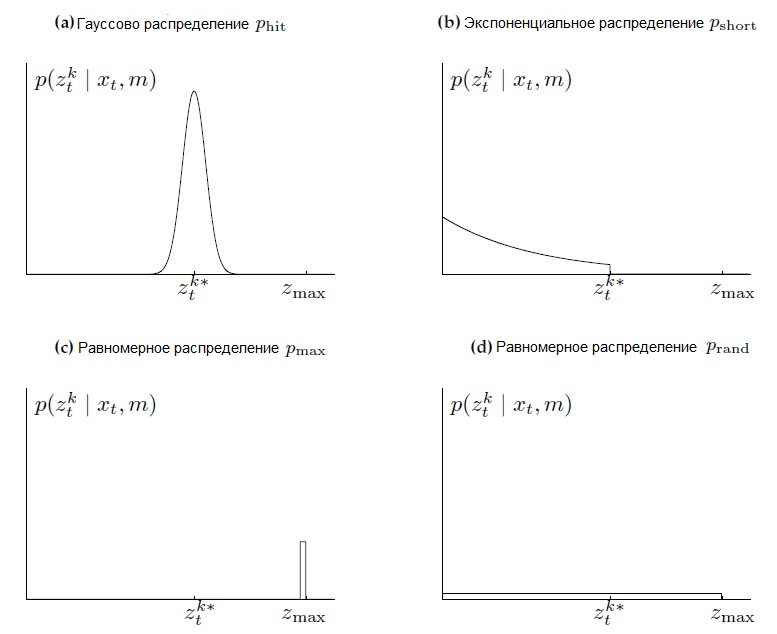
\includegraphics[width=1\linewidth]{63orig}}
	\caption{ (  Рис. 6.3 Компоненты модели датчика определения расстояния. На каждой схеме горизонтальная ось соответствует измерению $z_t^k$, а вертикальная - правдоподобию.)}
	\label{fig:63orig}
\end{figure}

1. \textbf{Верное измерение дистанции с локальным шумом измерений}. В идеальных условиях дальномер всегда измеряет верное расстояние до ближайшего объекта в поле измерения. Обозначим через $z^{k*}_t$ «истинное» расстояние до объекта, измеренное $z_t^k$. В картах на основе местоположения расстояние $z_t^{k*}$ можно определить, используя метод «бросания лучей» (ray casting), в картах на основе признаков они обычно получаются путём поиска ближайшего признака в конусе измерений. Однако, даже если датчик верно измеряет расстояние до ближайшего объекта, возвращаемое значение подвержено ошибке. Эта ошибка возникает в силу ограниченного разрешения дальномеров, атмосферных эффектов измеряющего сигнала и так далее.  

ШУМЫ ИЗМЕРЕНИЙ 

Этот вид \textit{шумов измерений} обычно моделируется узким гауссовым распределением с математическим ожиданием $z^{k*}_t$ и стандартным отклонением $\sigma_{hit}$. Обозначим гауссову функцию как $p_{hit}$. На Рис. 6.3a показана плотность $p_{hit}$  отдельного значения $z_t^{k*}$.\\

На практике значения измерений дальномера ограничены интервалом $[0; z_{max}]$, где $z_{max}$ - максимальное расстояние измерений. Отсюда, вероятность измерения задана в виде\\

(6.4) 
\begin{equation*}
p_{hit}(z_t^k|x_t,m)=\left\{
\begin{array}{ll}
\eta\, \mathcal N(z_t^k;z_t^{k*},\sigma_{hit}^2) & \mbox{ если }0\leq z_t^k\leq z_{max}\\
0 & \mbox{в других случаях}\\
\end{array}
\right.
\end{equation*}

где $z_t^{k*}$ вычисляется на основании $x_t$ и $m$ с помощью бросания лучей, а $\mathcal N(z_t^k;z_t^{k*},\sigma_{hit}^2)$
определяет одномерное нормальное распределение с математическим ожиданием $z_t^{k*}$ и стандартным отклонением $\sigma_{hit}$:

(6.5)
$$\mathcal N(z_t^k;z_t^{k*},\sigma_{hit}^2)=\frac{1}{\sqrt{2\pi\sigma_{hit}^2}}e^{-\frac{1}{2}\frac{(z_t^k - z_t^{k*})^2}{\sigma_{hit}^2}}$$

Нормализующий член $\eta$, оценочно\\

(6.6)
$$\eta=\left( \int_0^{z_{max}}\mathcal N(z_t^k;z_t^{k*},\sigma_{hit}^2)dz_t^k\right) ^{-1}$$

Стандартное отклонение $\sigma_{hit}$ является действительным параметром зашумления модели измерения. Мы обсудим стратегии установки этого параметра ниже. \\

\textbf{2. Неучтенные объекты.} Окружающие среды мобильных роботов изменчивы, хотя сами карты $m$ статические. В результате, объекты, отсутствующие на карте, могут заставить дальномеры выдавать неожиданно малые значения расстояний, по крайней мере, при сравнении с картой. Типичным примером таких движущихся объектов, которых нет на карте, являются люди, находящиеся в непосредственной близости от робота. Одним из способов обработки таких ситуаций является включение их в вектор состояния с последующей оценкой местоположения. Другим, гораздо более простым путём является включение их в шумы. 
При включении в шумы объекты, которых нет в модели, могут укорачивать измеренные расстояния $z_t^{k*}$, но неспособны их увеличивать.

Вероятность обнаружения неучтенных объектов уменьшается с расстоянием. Для примера, представим двух человек, которые независимо и с одинаковой вероятностью появляются в поле восприятия датчика движения. Расстояние до первого человека равно $r_1$, а до второго - $r_2$. Также допустим, что $r_1 < r_2$, без потери обобщения. Видно, что большую вероятность будет иметь измерение $r_1$, нежели $r_2$. При появлении первого человека показания датчика будут $r_1$. Для того, чтобы показания были $r_2$, должна сложиться ситуация, когда будет присутствовать только второй человек, а первый - отсутствовать.

Математически, вероятность измерения расстояния в таких ситуациях описывается \textit{экспоненциальным распределением}. Параметр этого распределения, $\lambda_{short}$, является внутренним параметром модели измерений. В соответствии с определением экспоненциального распределения, получаем следующее равенство для $p_{short}(z_t^k | x_t, m)$: \\

(6.7)
\begin{equation*}
p_{short}(z_t^k | x_t, m)=\left\{
\begin{array}{ll}
\eta\, \lambda_{short}\,e^{-\lambda_{short}z_t^k} & \mbox{ если }0\leq z_t^k\leq z_t^{k*}\\
0 & \mbox{в других случаях}\\
\end{array}
\right.
\end{equation*}

Как и в предыдущем случае, требуется нормализующий член $\eta$, поскольку экспонента ограничена интервалом $[0;z_t^{k*}]$. В силу того, что суммарная вероятность на этом интервале задана в виде 

(6.8)
\begin{equation*}
\begin{split}
\int_0^{z_t^{k*}}\lambda_{short}\,e^{-\lambda_{short}z_t^k}dz_t^k&=-e^{-\lambda_{short}z_t^{k*}}+e^{-\lambda_{short}0}\\
&=1-e^{-\lambda_{short}z_t^{k*}}
\end{split}
\end{equation*}

значение $\eta$ можно вывести, как:\\

(6.9)
$$\eta=\frac{1}{1-e^{-\lambda_{short}z_t^{k*}}}$$

На Рис. 6.3b эта плотность показана в графическом виде. Очевидно, что она экспоненциально уменьшается с расстоянием $z_t^k$.\\

\textbf{3. Отказы.} Иногда все препятствия одновременно "исчезают". Это часто происходит, например, с датчиками сонаров в результате зеркальных отражений. 
Отказы также случаются с лазерными дальномерами при сканировании чёрных, светопоглощающих объектов или же с некоторыми лазерными системами, которые неустойчиво работают при ярком солнечном свете.\\ 
ОТКАЗ ДАТЧИКА \\
Типичным результатом отказа датчика является возвращение показаний максимального расстояния, то есть датчик возвращает $z_{max}$. Такие события происходят достаточно часто, поэтому необходимо явно учитывать измерения максимального расстояния в модели измерений.

Смоделируем этот случай размещением точечной вероятности с центром в $z_{max}$:\\

(6.10)
\begin{equation*}
p_{max}(z_t^k | x_t, m)=I(z=z_{max})=\left\{
\begin{array}{ll}
1 & \mbox{ если } z=z_{max}\\
0 & \mbox{в других случаях}\\
\end{array}
\right.
\end{equation*}

Здесь была определена индикаторная функция, которая принимает значение 1, если аргумент имеет значение True, и 0 – в противном случае. Технически, $p_{max}$ не определяет функцию плотности вероятности, поскольку $p_{max}$ является дискретным распределением. Однако, это не должно нас волновать, ведь несуществующая функция плотности на математическую модель оценки вероятности измерения датчика не влияет. На наших схемах просто изобразим $p_max$ в виде очень узкого равномерного распределения с центром в $z_{max}$, представив, что такая плотность существует.

\begin{figure}[H]
	\center{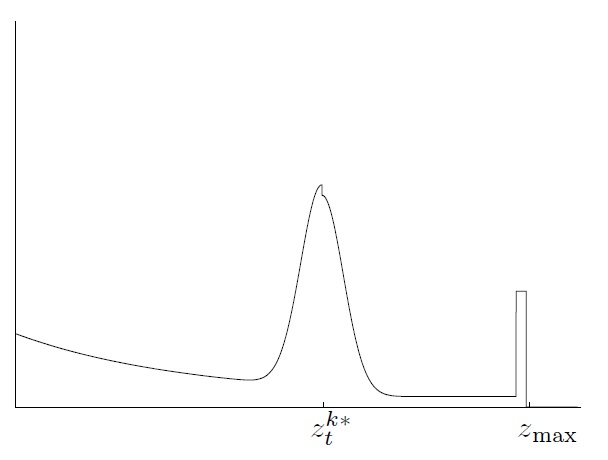
\includegraphics[width=1\linewidth]{64orig}}
	\caption{ (  Рис. 6.4  «Псевдовероятность» типичной смеси распределений $p(z_t^k | x_t, m)$.)}
	\label{fig:64orig}
\end{figure}

\textbf{4. Случайные измерения.} Наконец, дальномеры время от времени возвращают совершенно \textit{необъяснимые измерения.}\\
НЕОБЪЯСНИМЫЕ 
ИЗМЕРЕНИЯ \\ 
Так, сонары часто возвращают фантомные показания из-за отражения от стен или при перекрёстных наводках между различными датчиками. Для упрощения, такие измерения будут моделированы, используя равномерное распределение по всему диапазону измерений датчика $[0;z_{max}]$:\\

(6.11)
\begin{equation*}
p_{rand}(z_t^k | x_t, m)=\left\{
\begin{array}{ll}
\frac{1}{z_{max}} & \mbox{ если } 0\leq z_t^k\leq z_{max}\\
0 & \mbox{в других случаях}\\
\end{array}
\right.
\end{equation*}

На Рис. 6.3d показана плотность распределения $p_{rand}$.

Эти четыре разных распределения учтены в виде взвешенной средней, определённой параметрами $z_{hit}$, $z_{short}$, $z_{max}$ и $z_{rand}$, где $z_{hit} + z_{short} + z_{max} +z_{rand} = 1$.\\

(6.12)
\begin{minipage}{0.3\textwidth}
	\begin{equation*}
	p(z_t^k|x_t,m)=
	\left(\begin{array}{c}
	z_{hit}\\
	z_{short}\\
	z_{max}\\
	z_{rand}\\
	\end{array}\right)^T
	\hspace{2mm}
	\cdot \hspace{2mm}\left(\begin{array}{c}
	p_{hit}(z_t^k|x_t,m)\\
	p_{short}(z_t^k|x_t,m)\\
	p_{max}(z_t^k|x_t,m)\\
	p_{rand}(z_t^k|x_t,m)\\
	\end{array}\right)
	\end{equation*}
\end{minipage}

Типичная плотность вычисляется из линейной комбинации отдельных плотностей, показанных на Рис. 6.4 (с визуализацией распределения точечной вероятности $p_max$ в виде небольшой однородной плотности). Как может заметить читатель, основные характеристики всех четырёх базовых моделей все ещё присутствуют в этой комбинированной плотности. 

\begin{table}[H]
\begin{center}
\begin{tabular}{|l|}
\hline
{}\\
1: \hspace{3mm} Algorithm beam\_range\_finder\_model $(z_t,x_t,m):$ \\
{}\\
2:\hspace{7mm}$q=1$\\
3:\hspace{7mm}$\textit{for}\,k=1\,\textit{to}\,K\,\textit{do}$\\
4:\hspace{12mm}$\textit{вычислить }\,z_t^{k*}\,\textit{для измерения }\,z_t^k\,\textit{ используя метод бросания лучей}$\\
5:\hspace{12mm}$p=z_{hit}\cdot p_{hit}(z_t^k|x_t,m)+z_{short}\cdot p_{short} (z_t^k|x_t,m)$\\
6:\hspace{17mm}$+z_{max}\cdot p_{max}(z_t^k|x_t,m)+z_{rand}\cdot p_{rand} (z_t^k|x_t,m)$\\
7:\hspace{12mm}$q=q\cdot p$\\
8:\hspace{7mm}$\textit{return}\,q$\\
{}\\
\hline
\end{tabular}
\caption{(Таблица 6.1 Алгоритм для вычисления схожести сканирования расстояния $z_t$, допуская условную независимость между отдельными измерениями расстояния в проходе сканирования.)}
\end{center}
\end{table}

Модель дальномера реализована алгоритмом  beam\_range\_finder\_model в Таблице 6.1. На вход этой модели подаётся  полный проход сканирования $z_t$, положение робота $x_t$, и карта $m$. Во внешнем цикле (в строках 2 и 7) правдоподобия отдельных лучей датчика $z_t^k$ перемножаются, давая равенство (6.2). В строке 4 используется «метод бросания лучей» для вычисления расстояния отдельного измерения датчика с учётом шума. Вероятность каждого отдельного измерения расстояния $z^k_t$ вычисляется в строке 5, где выполняется смешивание плотностей из (6.12). После прохода по всем измерениям датчика $z_t^k$ в наборе $z_t$, алгоритм возвращает искомую вероятность $p(z_t | x_t, m)$.\\

\textbf{6.3.2 Настройка внутренних параметров модели}\\

Пока в нашем обсуждении не был освещён вопрос выбора различных параметров модели датчика. Эти параметры включают параметры смешивания $z_{hit}$, $z_{short}$, $z_{max}$, и $z_{rand}$, а также $\sigma_{hit}$ и $\lambda_{short}$. Обозначим набор всех внутренних параметров через $\varTheta$.
Очевидно, вероятность любого измерения датчика является функцией $\varTheta$. Поэтому, обсудим алгоритм для \textit{настройки параметров модели}.

Одним из способов определения внутренних параметров является анализ данных. На Рис. 6.5 показаны две серии из 10000 измерений, полученных мобильным роботом при передвижении в среде обычного офиса. 

\begin{figure}[H]
	\center{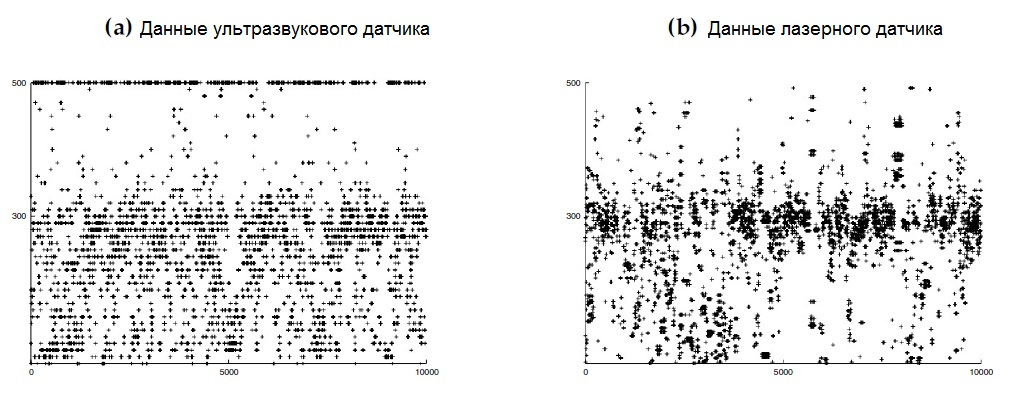
\includegraphics[width=1\linewidth]{65orig}}
	\caption{ ( Рис. 6.5 Типичные данные, полученные с (a) датчика сонара и (b) лазерного датчика расстояния в офисе для «истинного» расстояния 300 см и максимального расстояния 500 см.)}
	\label{fig:65orig}
\end{figure}

На обоих графиках изображены только измерения, предполагаемое значение которых приблизительно  равно 3 метрам (между 2,9 м и 3,1 м). На левом графике показаны данные для датчика сонара, а на правом – аналогичные данные лазерного датчика. В обоих случаях по оси $x$ показано число измерений (от 1 до 10000), а по оси $y$ – дальность, измеренная датчиком. 

Хотя большинство измерений обоих датчиков находится вблизи диапазона верных значений, поведение датчиков существенно различается. Ультразвуковой датчик, очевидно, гораздо больше подвержен шумам измерений и ошибкам обнаружения. Довольно часто он оказывается неспособен обнаружить имеющееся препятствие, возвращая максимальное расстояние. Напротив, лазерный дальномер значительно более точен, но и он, время от времени, возвращает неверные показания. 

Полностью применимым на практике способом регулировки внутренних параметров $\varTheta$ является их ручная установка таким образом, чтобы результирующая плотность была согласована с эмпирической картиной.
Другим, более надёжным способом является изучение значений параметров на основе настоящих данных.
Это достигается максимизацией правдоподобия опорного набора данных $Z = \left\lbrace z_i\right\rbrace $
относительно связанных положений $X = \left\lbrace x_i\right\rbrace $ и карты $m$, где каждая величина $z_i$ представляет собой актуальное измерение, $x_i$ - положение, из которого было получено измерение, а $m$ - карту. Правдоподобие данных $Z$ задано в виде\\

(6.13)
$$p(Z|X,m,\varTheta)$$

Нашей целью является определение внутренних параметров $\varTheta$, максимизирующих это правдоподобие.\\
ОЦЕНКА МАКСИМАЛЬНОГО ПРАВДОПОДОБИЯ\\ 
Оценивающая функция или алгоритм, максимизации правдоподобия обычно называются 
\textit{оценкой максимального правдоподобия}, ("ML estimator").

В Таблице 6.2 приводится алгоритм \textbf{learn\_intrinsic\_parameters} вычисления оценки максимального правдоподобия внутренних параметров. 

\begin{table}[H]
\begin{center}
\begin{tabular}{|l|}
\hline
{}\\
1: \hspace{3mm} Algorithm learn\_intrinsic\_parameters $(Z,X,m):$ \\
{}\\
2:\hspace{7mm}$\textit{repeat until convergence criterion satisfied}$\\
3:\hspace{12mm}$\textit{for all} \,z_i\,\textit{in}\,Z\,\textit{do}$\\
4:\hspace{17mm}$\eta={[ } p_{hit}(z_i|x_i,m)+p_{short}(z_i|x_i,m)$\\
\hspace{23mm}$ +p_{max}(z_i|x_i,m)+p_{rand}(z_i|x_i,m){] } ^{-1}$\\
5:\hspace{17mm}$\textit{calculate}\,z_i^*$\\
6:\hspace{17mm}$e_{i,hit}=\eta\,p_{hit}(z_i|x_i,m)$\\
7:\hspace{17mm}$e_{i,short}=\eta\,p_{short}(z_i|x_i,m)$\\
8:\hspace{17mm}$e_{i,max}=\eta\,p_{max}(z_i|x_i,m)$\\
9:\hspace{17mm}$e_{i,rand}=\eta\,p_{rand}(z_i|x_i,m)$\\
{}\\
10:\hspace{12mm}$z_{hit}=|Z|^{-1}\sum_i e_{i,hit}$\\
11:\hspace{12mm}$z_{short}=|Z|^{-1}\sum_i e_{i,short}$\\
12:\hspace{12mm}$z_{max}=|Z|^{-1}\sum_i e_{i,max}$\\
13:\hspace{12mm}$z_{rand}=|Z|^{-1}\sum_i e_{i,rand}$\\
14:\hspace{12mm}$\sigma_{hit}=\sqrt{\frac{1}{\sum_i e_{i,hit}}\sum_i e_{i,hit}(z_i-z_i^*)^2}$\\
15:\hspace{12mm}$\lambda_{short}=\frac{\sum_i e_{i,short}}{\sum_i e_{i,short}z_i}$\\
16:\hspace{7mm}$\textit{return}\,\varTheta=\{ z_{hit},z_{short},z_{max},z_{rand},\sigma_{hit},\lambda_{short}\}$\\
{}\\
\hline
\end{tabular}
\caption{(Таблица 6.2 Алгоритм обучения на основе данных для внутренних параметров модели датчика, использующего лучи. )}
\end{center}
\end{table}

Как будет показано ниже, алгоритм является примером метода  максимизации ожидания (expectation maximization -EM), итерационной процедуры оценки параметров максимального правдоподобия.

В начале работы алгоритма \textbf{learn\_intrinsic\_parameters} в Таблице 6.2 требуется качественная инициализация внутренних параметров $\sigma_{hit}$ и $\lambda_{short}$. В строках с 3 по 9 оцениваются вспомогательные переменные $e_{i,xxx}$ -  вероятности, что измерение  $z_i$ вызвано  причиной “xxx”, где “xxx” выбирается между четырьмя возможными шумами модели датчика: отражениями, короткими показаниями, максимальными показаниями и случайными шумами. Далее, в строках с 10 по 15, оцениваются внутренние параметры. Поскольку эти параметры являются функцией вычисленных ранее значений ожидания и их изменение вызывает изменение математического ожидания, алгоритм необходимо повторять. На практике процесс достаточно быстро завершаются, и, обычно, для получения хороших результатов хватает дюжины повторений. 

На Рис. 6.6 в графическом виде показаны четыре примера данных и модели измерения максимального правдоподобия, вычисленные с помощью \textbf{learn\_intrinsic\_parameters}. В первой строке показаны приближения к данным, полученным с помощью ультразвукового датчика. Во второй строке приведены графики двух функций, сгенерированных из данных лазерного дальномера. Столбцы соответствуют различным «истинным» расстояниям. Данные организованы в виде гистограмм и легко заметить разницу между графиками. Чем меньше расстояние $z_t^{k*}$, тем точнее измерение. Для обоих датчиков ширина гауссовых функций меньше для более близких измерений, чем для более удалённых. Вдобавок, лазерный дальномер более точен по сравнению с ультразвуковым датчиком, что хорошо видно из более узкого графика гауссиана и меньшего числа максимальных значений измерений. Другой важной особенностью является относительно высокое правдоподобие близких и случайных измерений. Эта большая по величине ошибка правдоподобия  является, одновременно, и преимуществом, и недостатком. С одной стороны, количество информации при каждом опросе датчика уменьшается из-за малой  разницы правдоподобия отражения и случайного измерения. С другой стороны, это делает модель менее подверженной не смоделированным \textit{систематическим} искажениям, например, появлению людей, которые перекрывают путь роботу в течение длительного времени. 

\begin{figure}[H]
	\center{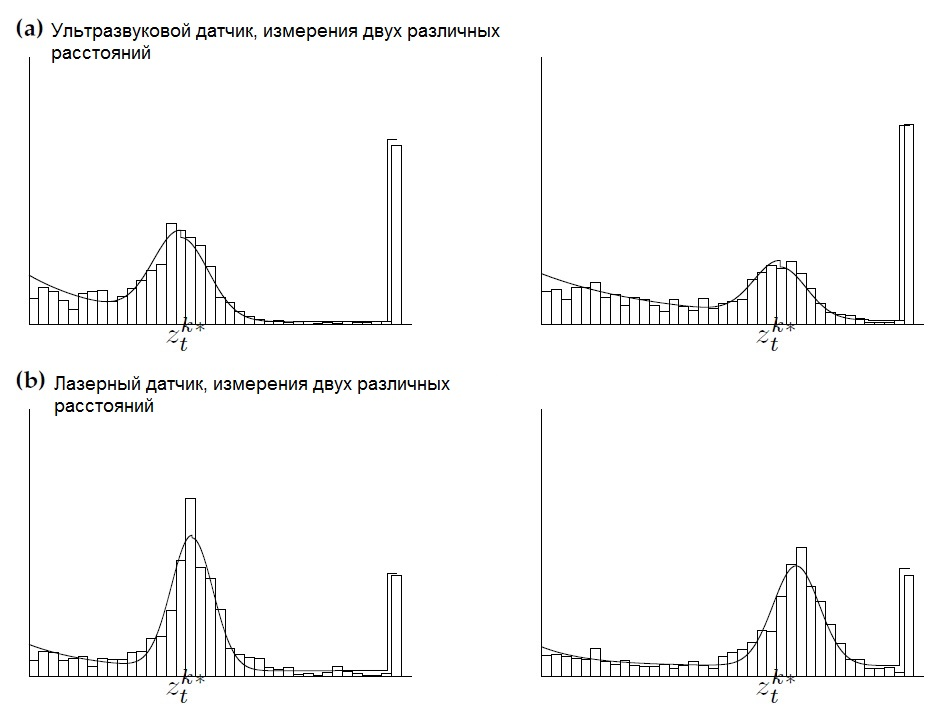
\includegraphics[width=0.9\linewidth]{66orig}}
	\caption{ (  Рис. 6.6 Приближение модели на основе лучей для (a) данных сонара и (b) данных лазера. Модели датчиков, показанные слева были получены методом максимального правдоподобия наборов данных на Рис. 6.5.)}
	\label{fig:66orig}
\end{figure}

На Рис. 6.7 показана в действии обученная модель датчика. На Рис. 6.7a показан проход сканирования шириной 180 градусов. Робот расположен в месте, предварительно полученном из карты занятости и его положение точно определено. На Рис. 6.7b изображена карта окружения с правдоподобностью $p(z_t | x_t, m)$  прохода сканирования расстояния, спроектированного в пространство $x-y$ (путём максимизации по ориентации $\varTheta$). Чем более тёмным цветом выделено местоположение, тем более оно вероятно. Как можно легко увидеть, все области с высоким правдоподобием расположены вдоль коридора. Неудивительно, поскольку отдельный проход сканирования лучше сохраняет геометрическую целостность в коридорах, нежели внутри комнат. Факт распределения массы вероятности вдоль коридора указывает на недостаточность отдельного прохода сканирования для определения точного положения робота. Это происходит, в основном, из-за симметричности коридора, а размещение апостериорного распределения в виде двух узких горизонтальных полос вызвано неизвестной ориентацией робота по направлению. Каждая полоса соответствует двум допустимым направлениям поворота робота. 

\textbf{6.3.3 Математический вывод модели на основе лучей}

Для вывода оценки методом максимального правдоподобия будет полезно ввести вспомогательную переменную $c_i$, так называемую переменную соответствия. Каждая $c_i$ может принимать одно из четырёх значений:  близкое, максимальное, случайное расстояние и отражение, что соответствует четырём возможным механизмам, создающим измерение $z_i$.

\begin{figure}[H]
	\center{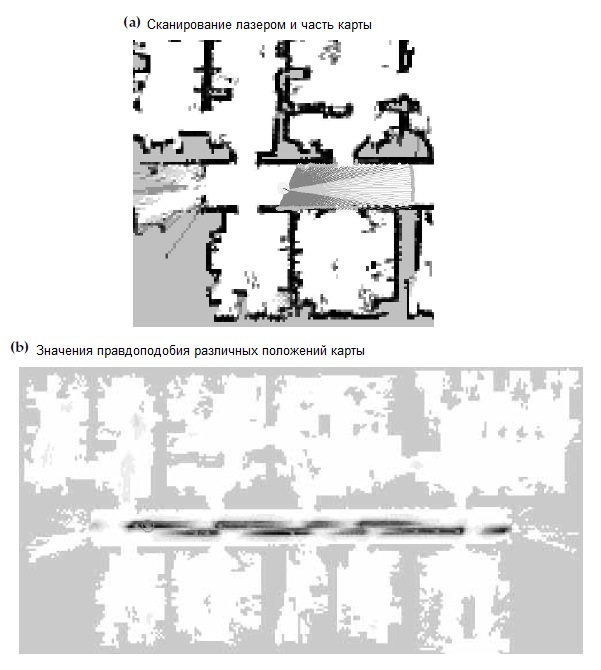
\includegraphics[width=0.9\linewidth]{67orig}}
	\caption{ (  Рис. 6.7 Вероятностная модель восприятия: (a) Проход сканирования расстояния лазером, в проекции на предварительно созданную карту $m$. (b) Оценка правдоподобия $p(z_t | x_t, m)$, всех местоположений $x_t$, спроектированная на карту (показана серым). Чем темнее местоположение, тем выше вероятность $p(z_t | x_t, m)$.)}
	\label{fig:67orig}
\end{figure}

Для начала разберём случай, когда $c_i$ неизвестны, но известно, каким из четырёх указанных выше механизмов вызывается каждое измерение $z_i$. На основе значений $c_i$, можно разложить $Z$ на четыре непересекающихся множества, $Z_{hit}$, $Z_{short}$, $Z_{max}$, и $Z_{rand}$, которые вместе и образуют полный набор данных $Z$. Оценка максимального правдоподобия для внутренних параметров $z_{hit}$, $z_{short}$, $z_{max}$, и $z_{rand}$ представляет просто нормализованные соотношения:\\

(6.14)
\begin{minipage}{0.3\textwidth}
	\begin{equation*}
	\left(\begin{array}{c}
	z_{hit}\\
	z_{short}\\
	z_{max}\\
	z_{rand}\\
	\end{array}\right)
	\hspace{2mm}
	=
	\hspace{2mm}
	|Z|^{-1}
	\hspace{2mm}\left(\begin{array}{c}
	|Z_{hit}|\\
	|Z_{short}|\\
	|Z_{max}|\\
	|Z_{rand}|\\
	\end{array}\right)
	\end{equation*}
\end{minipage}

Оставшиеся внутренние параметры, $\sigma_{hit}$ и $\lambda_{short}$, получаются следующим образом.
Для набора данных $Z_{hit}$, получим из (6.5)

(6.15)
\begin{equation*}
\begin{split}
p(Z_{hit}|X,m,\varTheta)&=\prod_{z_i\in Z_{hit}}p_{hit}(z_i|x_i,m,\varTheta)\\
&=\prod_{z_i\in Z_{hit}}\frac{1}{\sqrt{2\pi\sigma_{hit}^2}}e^{-\frac{1}{2}\frac{(z_i-z_t^*)^2}{\sigma_{hit}^2}}
\end{split}
\end{equation*}

Здесь $z_i^*$ - «истинное» расстояние, вычисленное из положения $x_i$ и карты $m$. Классическим способом оценки правдоподобия является максимизация логарифма правдоподобия, а не самого значения правдоподобия. Логарифм является строго монотонной функцией, поэтому максимум логарифма правдоподобия является и максимумом самого правдоподобия. Логарифм правдоподобия задан в виде\\

(6.16)
$$\log p(Z_{hit}|X,m,\varTheta)=\sum_{z_i\in Z_{hit}}\left[ -\frac{1}{2}\log2\pi\sigma_{hit}^2-\frac{1}{2}\frac{(z_i-z_i^*)^2}{\sigma_{hit}^2}\right] $$

и легко преобразуется следующим образом\\

(6.17)
\begin{equation*}
\begin{split}
\log p&(Z_{hit}|X,m,\varTheta)\\
&=-\frac{1}{2}\sum_{z_i\in Z_{hit}}\left[ \log2\pi\sigma_{hit}^2+\frac{(z_i-z_i^*)^2}{\sigma_{hit}^2}\right] \\
&=-\frac{1}{2}\left[ |Z_{hit}|\log2\pi+2|Z_{hit}|\log\sigma_{hit}+\sum_{z_i\in Z_{hit}}\frac{(z_i-z_i^*)^2}{\sigma_{hit}^2}\right] \\
&=\text{const.}-|Z_{hit}|\log\sigma_{hit}-\frac{1}{2\sigma_{hit}^2}\sum_{z_i\in Z_{hit}}(z_i-z_i^*)^2
\end{split}
\end{equation*}

Производная этого выражения по внутренним параметрам $\sigma_{hit}$ выглядит следующим образом:

(6.18)
$$\frac{\partial\log p(Z_{hit}|X,m,\varTheta)}{\partial\sigma_{hit}}=-\frac{|Z_{hit}|}{\sigma_{hit}}+\frac{1}{\sigma_{hit}^3}\sum_{z_i\in Z_{hit}}(z_i-z_i^*)^2$$

Максимум логарифма правдоподобия получается установкой этой производной в нуль. Отсюда и решение оценки методом максимального правдоподобия. \\

(6.19)
$$\sigma_{hit}=\sqrt{\frac{1}{|Z_{hit}|}\sum_{z_i\in Z_{hit}}(z_i-z_i^*)^2}$$

Оценка оставшегося внутреннего параметра $\lambda_{short}$ выполняется практически таким же образом. Апостериорное распределение $Z_{short}$ задано в виде\\

(6.20)
\begin{equation*}
\begin{split}
p(Z_{short}|X,m,\varTheta)&=\prod_{z_i\in Z_{short}}p_{short}(z_i|x_i,m)\\
&=\prod_{z_i\in Z_{short}}\lambda_{short}\,e^{-\lambda_{short}z_i}
\end{split}
\end{equation*}

Логарифм выражения\\

(6.21)
\begin{equation*}
\begin{split}
\log p(Z_{short}|X,m,\varTheta)&=\sum_{z_i\in Z_{short}}\log\lambda_{short}-\lambda_{short}z_i\\
&=|Z_{short}|\log\lambda_{short}-\lambda_{short}\sum_{z_i\in Z_{short}}z_i
\end{split}
\end{equation*}

Первая производная этого выражения по отношению к внутреннему параметру $\lambda_{short}$ выглядит следующим образом:\\

(6.22)
$$\frac{\partial\log p(Z_{short}|X,m,\varTheta)}{\partial\lambda_{short}}=\frac{|Z_{short}|}{\lambda_{short}}-\sum_{z_i\in Z_{short}}z_i$$

Установка производной в нуль даёт оценку максимального внутреннего правдоподобия $\lambda_{short}$\\

(6.23)
$$\lambda_{short}=\frac{|Z_{short}|}{\sum_{z_i\in Z_{short}}z_i}$$

Для вычисления производной подразумевается знание параметров $c_i$. Обобщим этот случай для ситуации, когда $c_i$ неизвестно. Как будет показано, результирующая задачи оценка максимизации правдоподобия не имеет решения в закрытом виде. Однако, можно предложить метод вычисления ожидания $c_i$ в цикле из двух шагов, с последующим вычислением внутренних параметров модели по этим ожиданиям.\\ 
АЛГОРИТМ МАКСИМИЗАЦИИ ОЖИДАНИЯ\\
Как было отмечено, результирующий алгоритм является экземпляром \textit{алгоритма максимизации ожидания} обычно сокращаемом до EM.

Чтобы вывести EM, будет уместно сначала определить правдоподобие данных $Z$:\\

(6.24)
\begin{equation*}
\begin{split}
\log p&(Z|X,m,\varTheta)\\
&=\sum_{z_i\in Z}\log p(z_i|x_i,m,\varTheta)\\
&=\sum_{z_i\in Z_{hit}}\log p_{hit}(z_i|x_i,m)+\sum_{z_i\in Z_{short}}\log p_{short}(z_i|x_i,m)\\
&+\sum_{z_i\in Z_{max}}\log p_{max}(z_i|x_i,m)+\sum_{z_i\in Z_{rand}}\log p_{rand}(z_i|x_i,m)
\end{split}
\end{equation*}

Это выражение может быть переписано с использованием переменных $c_i$:\\

(6.25)
\begin{equation*}
\begin{split}
\log p(Z|X,m,\varTheta)=&\sum_{z_i\in Z}I(c_i=\text{hit})\log p_{hit}(z_i|x_i,m)\\
&+I(c_i=\text{short})\log p_{short}(z_i|x_i,m)\\
&+I(c_i=\text{max})\log p_{max}(z_i|x_i,m)\\
&+I(c_i=\text{rand})\log p_{rand}(z_i|x_i,m)
\end{split}
\end{equation*}

где $I$ – индикаторная функция. Поскольку значения $c_i$ неизвестны, остаётся только интегрировать их. Другими словами, с помощью EM максимизируется ожидание $E[\log\, p(Z | X, m, \varTheta)]$ по неизвестным переменным $c_i$:\\

(6.26)
\begin{equation*}
\begin{split}
E[\log\, &p(Z|X,m,\varTheta)]\\
&=\sum_i p(c_i=\text{hit})\log p_{hit}(z_i|x_i,m)+p(c_i=\text{short})\log p_{short}(z_i|x_i,m)\\
&+p(c_i=\text{max})\log p_{max}(z_i|x_i,m)+p(c_i=\text{rand})\log p_{rand}(z_i|x_i,m)\\
&=:\sum_i e_{i,hit}\log p_{hit}(z_i|x_i,m)+e_{i,short}\log p_{short}(z_i|x_i,m)\\
&+e_{i,max}\log p_{max}(z_i|x_i,m)+e_{i,rand}\log p_{rand}(z_i|x_i,m)
\end{split}
\end{equation*}

Переменная $e$ определяется указанным выше способом. Это выражение максимизируется в два шага. На первом шаге будем считать, что внутренние параметры $\sigma_{hit}$ и $\lambda_{short}$ заданы изначально, и вычислим математическое ожидание по переменной $c_i$.\\

(6.27)
\begin{minipage}{0.3\textwidth}
\begin{equation*}
	\left(\begin{array}{c}
	e_{i,hit}\\
	e_{i,short}\\
	e_{i,max}\\
	e_{i,rand}\\
	\end{array}\right)
	\hspace{2mm}
	:=
	\hspace{2mm}
	\left(\begin{array}{c}
	p(c_i=\text{hit})\\
	p(c_i=\text{short})\\
	p(c_i=\text{max})\\
	p(c_i=\text{rand})\\
	\end{array}\right)
	\hspace{2mm}
	=
	\hspace{2mm}
	\eta\,
	\left(\begin{array}{c}
	p_{hit}(z_i|x_i,m)\\
	p_{short}(z_i|x_i,m)\\
	p_{max}(z_i|x_i,m)\\
	p_{rand}(z_i|x_i,m)\\
	\end{array}\right)
\end{equation*}
\end{minipage}

Нормализующий член задан в виде\\

(6.28)
$$\eta=[p_{hit}(z_i|x_i,m)+p_{short}(z_i|x_i,m)
+p_{max}(z_i|x_i,m)+p_{rand}(z_i|x_i,m)]^{-1}$$

Этот шаг называется "шаг-E", указывая на вычисление математического ожидания латентных переменных $c_i$. Оставшийся шаг теперь очевиден, поскольку ожидания выражают зависимости между разными компонентами модели датчика. Во-первых, заметим, что параметры смеси ML представляют собой просто нормализованные ожидания\\

(6.29)
\begin{minipage}{0.3\textwidth}
	\begin{equation*}
	\left(\begin{array}{c}
	z_{hit}\\
	z_{short}\\
	z_{max}\\
	z_{rand}\\
	\end{array}\right)
	\hspace{2mm}
	=
	\hspace{2mm}
	|Z|^{-1}\sum_i
	\left(\begin{array}{c}
	e_{i,hit}\\
	e_{i,short}\\
	e_{i,max}\\
	e_{i,rand}\\
	\end{array}\right)
	\end{equation*}
\end{minipage}

Параметры ML $\sigma_{hit}$ и $\lambda_{short}$ получаются аналогично, заменой жёсткого присваивания значений в (6.19) и (6.23) присваиванием взвешенных значений.\\

(6.30)
$$\sigma_{hit}=\sqrt{\frac{1}{\sum_{z_i\in Z}e_{i,hit}}\sum_{z_i\in Z}e_{i,hit}(z_i-z_i^*)^2}$$

и\\

(6.31)
$$\lambda_{short}=\frac{\sum_{z_i\in Z}e_{i,short}}{\sum_{z_i\in Z}e_{i,short}z_i}$$\\

\textbf{6.3.4 Практические соображения}\\

На практике, вычисление плотностей всех показаний датчиков может быть вычислительно затруднено. Например, лазерные сканеры расстояния часто возвращают сотни значений за проход, выполняя несколько проходов в секунду. Поскольку для каждого луча сканирования необходимо выполнить операцию «бросания луча» в каждое возможное местоположение, интеграцию текущего прогноза в проход сканирования в реальном времени выполнить невозможно. Обычным способом решения задачи является включение в расчёт только ограниченного набора измерений (например, восьми равномерно распределенных измерений на проход сканирования лазера вместо 360). Такой подход имеет важное дополнительное преимущество. Поскольку соседние лучи прохода сканирования часто не являются независимыми, процесс оценки состояния становится менее подвержен коррелированному шуму соседних измерений.

При выраженной зависимости между соседними измерениями применение модели ML может привести робота к излишней самоуверенности и совершенно неоптимальным результатам оценки местоположения. Один простой приём, позволяющий этого избежать, состоит в замене $p(z_t^k | x_t, m)$ более «слабой» версией $p(z_t^k | x_t, m)^\alpha$ при $\alpha < 1$. Идея состоит в уменьшении, на коэффициент $\alpha$, информации, извлечённой из измерения датчика (логарифм этой вероятности задан в виде $\alpha\log\, p(z_t^k | x_t, m)$). Другая возможность, которая будет только упомянута здесь, это выяснение внутренних параметров в контексте приложения. Например, в мобильной локализации возможно обучить модель внутренних параметров градиентным спуском для получения хороших результатов локализации в течение нескольких тактов времени. 
Такая методология с несколькими шагами существенно отличается от метода оценки максимального правдоподобия, описанного выше. В практическом применении этот метод может дать отличные результаты. (Thrun, 1998a).

Самой затратной, в вычислительном смысле, частью моделей на основе лучей является операция бросания луча. Затраты на вычисление $p(z_t | x_t, m)$ могут быть существенно уменьшены предварительным кэшированием результатов работы алгоритма бросания лучей и хранением их в памяти, заменив, таким образом, операцию бросания лучей значительно более быстрым проходом по таблице. Очевидной реализацией этой идеи является разбиение пространства состояний на трехмерную сетку с мелкой ячейкой и вычисление диапазонов $z_t^{k*}$ для каждой ячейки сети. Эта идея уже была описана в Главе 4.1 и, в зависимости от разрешения сетки, требования к памяти могут оказаться весьма существенными. В задаче локализации мобильного робота пространство с разрешением сетки 15 см на 2 градуса хорошо показывает себя в задачах локализации в замкнутом пространстве. Такая карта хорошо помещается в памяти средних по мощности компьютеров, показывая производительность на порядок лучше бросания лучей в реальном времени.\\

\textbf{6.3.5 Ограничения модели лучей}\\

Модель датчика на основе лучей, хотя и пересекается  с геометрией и физикой дальномеров, имеет два важных недостатка.

В частности, модель на основе лучей  недостаточно гладкая. В загромождённых средах с множеством малых препятствий распределение $p(z_t^k | x_t, m)$ может быть очень негладким по $x_t$. Для примера возьмём среду с множеством стульев и столов (скажем,  конференц-зал). Робот, показанный в Главе 1, сможет воспринимать ножки этих препятствий. Очевидно, небольшие изменения положения робота $x_t$ могут оказать огромное влияние на верное определение расстояния лучом датчика. В результате, модель измерения $p(z_t^k | x_t, m)$ сильно прерывиста по $x_t$. В частности, затрагивается параметр направления поворота $\theta_t$, поскольку малые изменения направления могут вызвать большие смещения в пространстве  $x-y$ на расстояниях измерения.

Недостаток гладкости имеет два следствия. Во-первых, любое примерное представление подвержено опасности потери корректного состояния, поскольку ближайшие состояния могут иметь радикально различные апостериорные правдоподобия. Это накладывает ограничения на точность аппроксимации, которые могут привести к увеличению результирующей апостериорной ошибки. Во-вторых, методы поиска экстремума для нахождения наиболее вероятного состояния в условиях с большим количеством локальных минимумов в негладких моделях страдают от проблемы локального минимума. 

Модель на основе лучей также является вычислительно затратной. Оценка $p(z_t^k | x_t, m)$ каждого единичного измерения датчика $z_t^k$ включает бросание лучей, что требует достаточной вычислительной мощности. Как было отмечено выше, задача может быть частично упрощена предварительным вычислением диапазонов на дискретной сетке пространства положений.
Такой подход смещает акцент вычислений на начальную оффлайновую фазу, ускоряя работу алгоритма. Однако, результирующие таблицы очень велики, поскольку покрывают значительные участки трехмерного пространства. В силу этого, предварительный расчёт расстояний является вычислительно затратным и требует значительного объёма памяти.\\

\textbf{6.4 Поля правдоподобия для датчиков расстояния}\\

\textbf{6.4.1 Общий алгоритм}\\

ПОЛЕ ПРАВДОПОДОБИЯ\\
Опишем альтернативную модель под названием \textit{поле правдоподобия}, которая обходит эти ограничения, но внятного физического объяснения не имеет.
Фактически, это специализированный алгоритм, который вовсе не обязательно вычисляет условную вероятность относительно применимой генеративной модели физики датчиков, но на практике работает хорошо. Результирующие апостериорные распределения значительно более гладкие даже в загромождённом пространстве, а вычисления – более эффективные.

Ключевая идея состоит в проекции конечных точек прохода сканирования датчика $z_t$ в глобальное координатное пространство карты. Чтобы это сделать, необходимо определить, как именно в глобальной системе координат расположена локальная система отсчёта робота, откуда начинается луч датчика $z_k$ и куда он направлен. Как обычно, пусть $x_t = (x\,y\,\theta)^T$ определяет положение робота в момент времени $t$.
Сохраняя двухмерное представление окружающего мира, определим фиксированное относительное положение датчика робота, локальную координатную систему $(x_{k,sens}\, y_{k,sens})^T$, угловое положение луча датчика относительно направления робота $\theta_{k,sens}$. Эти значения зависят от типа датчика. Конечная точка измерения $z_t^k$ проектируется в глобальную систему координат с помощью очевидного тригонометрического преобразования.\\

(6.32)\\
 
\begin{minipage}{0.2\textwidth}
	\begin{equation*}
	\left(\begin{array}{c}
	x_{z_t^k}\\
	y_{z_t^k}\\
	\end{array}\right)
	=
	\left(\begin{array}{c}
	x\\
	y\\
	\end{array}\right)
	+
	\left(\begin{array}{c}
	\cos\theta\,\,-\sin\theta\\
	\sin\theta\,\,\,\,\,\cos\theta\\
	\end{array}\right)
	\left(\begin{array}{c}
	x_{k,sens}\\
	y_{k,sens}\\
	\end{array}\right)
	+z_t^k
	\left(\begin{array}{c}
	\cos(\theta+\theta_{k,sens})\\
	\sin(\theta+\theta_{k,sens})\\
	\end{array}\right)
	\end{equation*}
\end{minipage}\\

Эти координаты имеют смысл только для измерения, при котором датчик обнаруживает препятствие. 
Если датчик расстояния выдаёт максимальное значение $z_t^k = z_{max}$, координаты не имеют значения в физическом мире (хотя измерение и содержит информацию). В модели измерения на основе поля правдоподобия  показания максимального расстояния просто отбрасываются.

Аналогично модели на основе лучей, обсуждаемой выше, будут приниматься во внимание три источника зашумления и неопределённости: \\
\begin{figure}[H]
	\center{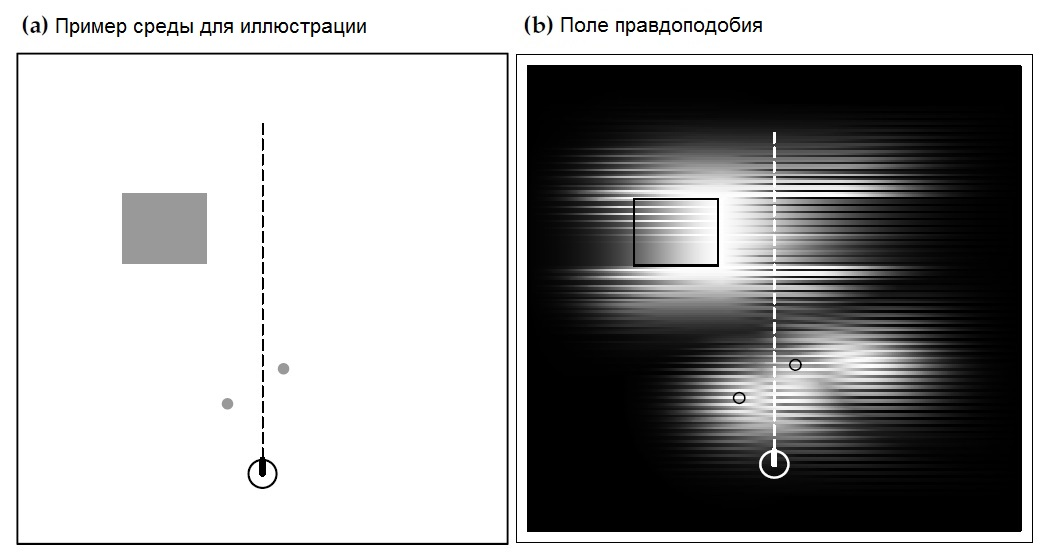
\includegraphics[width=1\linewidth]{68orig}}
	\caption{ (  Рис. 6.8 (a) Модельная среда с тремя препятствиями (выделены серым). Робот, расположенный внизу схемы, получает измерение $z_t^k$, обозначенное пунктиром. (b) Поле правдоподобия для данной конфигурации препятствий: чем темнее местоположение,	тем менее вероятно обнаружение препятствия в этой точке. Вероятность $p(z_t^k | x_t, m)$ для отдельного луча датчика показана на Рис. 6.9.
		)}
	\label{fig:68orig}
\end{figure}

\begin{figure}[H]
	\center{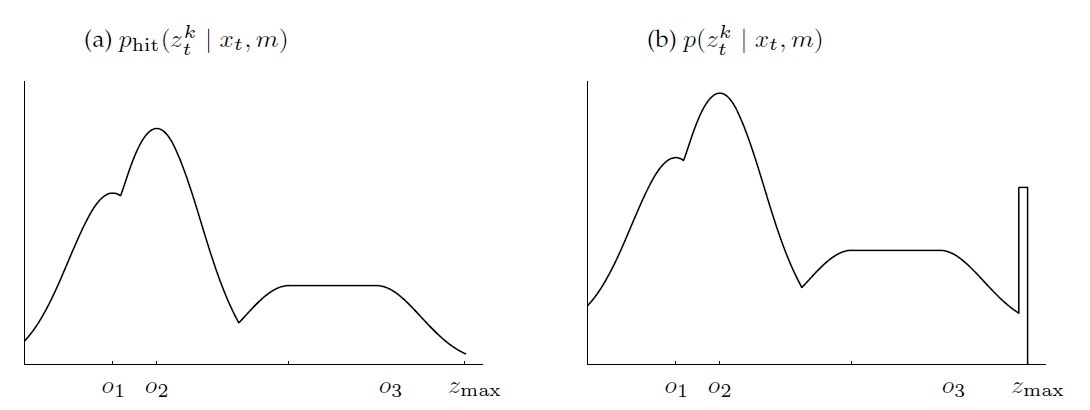
\includegraphics[width=1\linewidth]{69orig}}
	\caption{ (  Рис. 6.9 (a) Вероятность $p_{hit}(z_t^k)$ как функция измерения $z_t^k$, для ситуации, показанной на Рис. 6.8. Здесь луч датчика проходит по трём препятствиям с ближайшими точками $o_1$, $o_2$, и $o_3$, соответственно. (b) Вероятность датчика $p(z_t^k | x_t, m)$, полученная для ситуации на Рис. 6.8, двумя дополнительными равномерными распределениями.)}
	\label{fig:69orig}
\end{figure}

\textbf{1. Шумы измерения}. Шум при измерении смоделирован гауссовыми распределениями. В пространстве $x-y$ для этого требуется найти на карте ближайшее препятствие. Для начала просто определим  евклидово расстояние между 
координатами измерения $(x_{z^k_t}\,y_{z^k_t})^T$ и ближайшим объектом на карте $m$. Тогда вероятность измерения датчика будет задано гауссовой функцией с нулевым центром, учитывающей шумы датчика:\\

(6.33)
$$p_{hit}(z_t^k|x_t,m)=\varepsilon_{\sigma_{hit}}(\textit{dist})$$

На Рис. 6.8a показана карта, а на Рис. 6.8b - соответствующее гауссово правдоподобие для точек измерения $(x_{z^k_t}\,y_{z^k_t})^T$ в двухмерном пространстве. Чем более светлым цветом помечено местоположение, тем более вероятно измерение объекта с помощью датчика расстояния. Теперь плотность $p_{hit}$ получается пересечением (и нормализацией) поля правдоподобия  осью датчика, обозначенной пунктиром 6.8. Результирующая функция показана на Рис. 6.9a.\\

\textbf{2. Отказы.} Как и ранее, предположим, что показания максимального расстояния имеют выраженное большое правдоподобие и снова смоделируем это с помощью точечного распределения $p_{max}$.\\

\textbf{3. Необъяснимые случайные измерения.} Наконец, для моделирования случайного шума измерения используется однородное распределение $p_{rand}$.\\

Аналогично модели датчика на основе лучей, искомая вероятность $p(z_t^k | x_t, m)$ объединяет все три распределения:\\

(6.34)
$$z_{hit}\cdot p_{hit}+z_{rand}\cdot p_{rand}+z_{max}\cdot p_{max}$$

используя уже знакомое смешивание весов $z_{hit}$, $z_{rand}$, и $z_{max}$. На Рис. 6.9b показан пример результирующего распределения $p(z_t^k | x_t, m)$ вдоль луча измерения. Будет легко показать, что это распределение объединяет $p_{hit}$, как показано на Рис. 6.9a, с распределениями $p_{max}$ и $p_{rand}$. Большая часть сказанного о настройке параметров смешивания справедливо и для новой модели датчика. Параметры можно настраивать вручную или использовать обученный алгоритм смешивания.
Отображение наподобие показанного на Рис. 6.8b, показывает правдоподобие обнаружения препятствия в виде функции глобальных координат $x-y$ и называется \textit{полем правдоподобия}.

В Таблице 6.3 предлагается алгоритм вычисления вероятности измерений с использованием поля правдоподобия. Читателю уже должен быть знаком внешний цикл, в котором выполняется перемножение отдельных значений $p(z_t^k | x_t, m)$, подразумевая независимость между шумами в разных лучах датчика. В строке 4 проверяется не является ли измерение дальности максимальным, и, если да, такое значение отбрасывается. В строках с 5 по 8 происходит интересное преобразование. Сначала вычисляется расстояние до ближайшего препятствия (строка 7), а затем результирующее правдоподобие получается в строке 8 смешением нормального и равномерного распределений. Как и прежде, функцией \textbf{prob}$(dist, \sigma_{hit})$ вычисляется вероятность $dist$ под гауссовой функцией с нулевым математическим ожиданием и стандартным отклонением $\sigma_{hit}$.

\begin{table}[H]
\begin{center}
\begin{tabular}{|l|}
\hline
{}\\
1: \hspace{3mm} Algorithm likelihood\_field\_range\_finder\_model $(z_t,x_t,m):$ \\
{}\\
2:\hspace{7mm}$q=1$\\
3:\hspace{7mm}$\textit{for all} \,k\,\textit{do}$\\
4:\hspace{12mm}$\textit{if}\,z_t^k\neq z_{max}$\\
5:\hspace{17mm}$x_{z_t^k}=x+x_{k,sens}\cos\theta-y_{k,sens}\sin\theta+z_t^k\cos(\theta+\theta_{k,sens})$\\
6:\hspace{17mm}$y_{z_t^k}=y+y_{k,sens}\cos\theta+x_{k,sens}\sin\theta+z_t^k\sin(\theta+\theta_{k,sens})$\\
7:\hspace{17mm}$\textit{dist}=\underset{x',y'}{\min}\left\lbrace \sqrt{(x_{z_t^k}-x')^2+(y_{z_t^k}-y')^2}|\langle x',y'\rangle\,\text{occupied in \textit{m}}\right\rbrace $\\
8:\hspace{17mm}$q=q\cdot(z_{hit}\cdot\text{\textbf{prob}}(dist,\sigma_{hit})+\frac{z_{random}}{z_{max}})$\\
9:\hspace{7mm}$\textit{return}\,q$\\
{}\\
\hline
\end{tabular}
\caption{(Таблица 6.3 Алгоритм вычисления правдоподобия датчика расстояния на основе евклидова расстояния до ближайшего соседа. Функция \textbf{prob}$(\textit{dist}, \sigma_{hit})$ вычисляет вероятность расстояния под гауссовым распределением с нулевым математическим ожиданием и стандартным отклонением $\sigma_{hit}$ )}
\end{center}
\end{table}

Поиск ближайшего соседа на карте (строка 7) является самой затратной операцией в алгоритме \textbf{likelihood\_field\_range\_finder\_model}. Для ускорения поиска целесообразно предварительно вычислить поле правдоподобия, чтобы вычисление вероятности измерения сводилось к преобразованию координат с последующим просмотром таблицы. Конечно, при использовании дискретной сетки результат поиска достаточно приблизителен, поэтому может вернуть неверные координаты препятствия. Однако, эффект вероятности $p(z_t^k | x_t, m)$ обычно мал даже для достаточно грубых сеток.\\ 

\textbf{6.4.2 Обобщения}\\

Ключевым преимуществом модели поля правдоподобия над моделью на основе лучей, обсуждаемой раньше, является её гладкость. В силу гладкости функции евклидова расстояния, малые измерения положения робота $x_t$ оказывают лишь небольшой эффект на результирующее распределение $p(z_t^k | x_t, m)$. Другим ключевым преимуществом является выполнение предварительного расчёта в 2D вместо 3D, что уменьшает размер данных.

Такая модель имеет три главных недостатка. Во-первых, она неспособна явно моделировать людей и другие динамические процессы, способные вызвать слишком малые показания. 
Во-вторых, датчики в ней воспринимаются, как если бы они могли «видеть сквозь стены». Это происходит в результате замены операции бросания лучей функцией ближайшего соседа, неспособной определить пересечение пути к точке с препятствием. В-третьих, такой подход не принимает во внимание неопределённость карты. В частности, невозможно обработать неизвестные области, для которых карта не определена или же полностью неизвестна.

\begin{figure}[H]
	\center{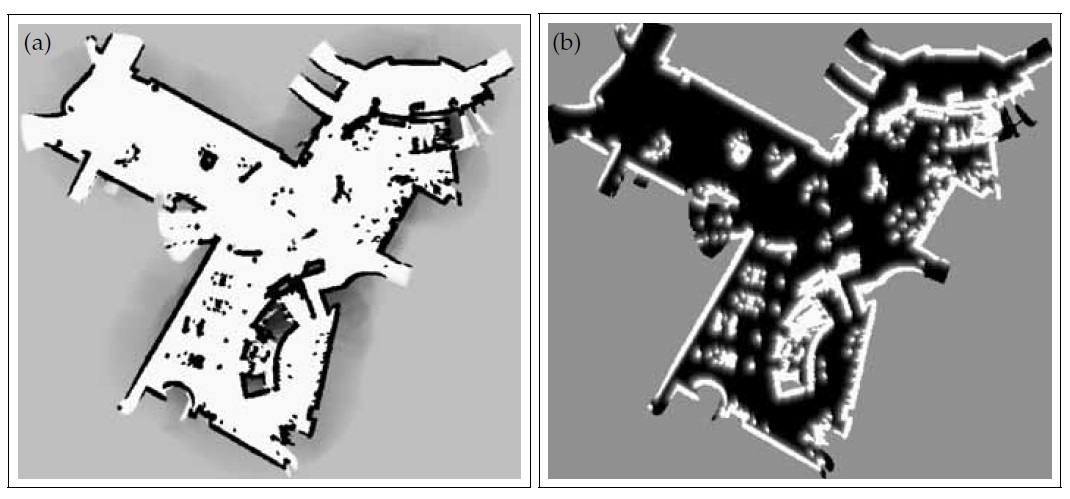
\includegraphics[width=0.85\linewidth]{610orig}}
	\caption{ (  Рис. 6.10 (a) Карта сетки занятости технического музея Сан-Хосе, (b) предварительное вычисленное поле правдоподобия.)}
	\label{fig:610orig}
\end{figure}

Основной алгоритм \textbf{likelihood\_field\_range\_finder\_model} может быть обобщён для минимизации эффекта этих ограничений. Например, возможно отсортировать значения занятости на карте по трём категориям: \textit{занято}, \textit{свободно}, и \textit{неизвестно}, а не только по первым двум. Когда измерение датчика $z_t^k$ попадает в категорию "неизвестно", ее вероятность $p(z_t^k | x_t, m)$ считается постоянной со значением $\frac{1}{z_{max}}$. Результирующая вероятностная модель достаточно груба, поскольку подразумевает, что в неизвестном пространстве каждое измерение датчика равновероятно.

На Рис. 6.10 показана карта и соответствующее ей поле правдоподобия. Как и прежде, выделение серым цветом местоположения $x-y$ обозначает правдоподобие получения показаний датчика в данной точке. Читатель может заметить, что расстояние до ближайшего препятствия применимо только \textit{внутри} карты, что соответствует обследованной территории. Вне карты правдоподобность $p(z_t^k | x_t, m)$ постоянна. В целях вычислительной эффективности полезно предварительно вычислить ближайшего соседа, используя мелкую двухмерную сетку.

\begin{figure}[H]
	\center{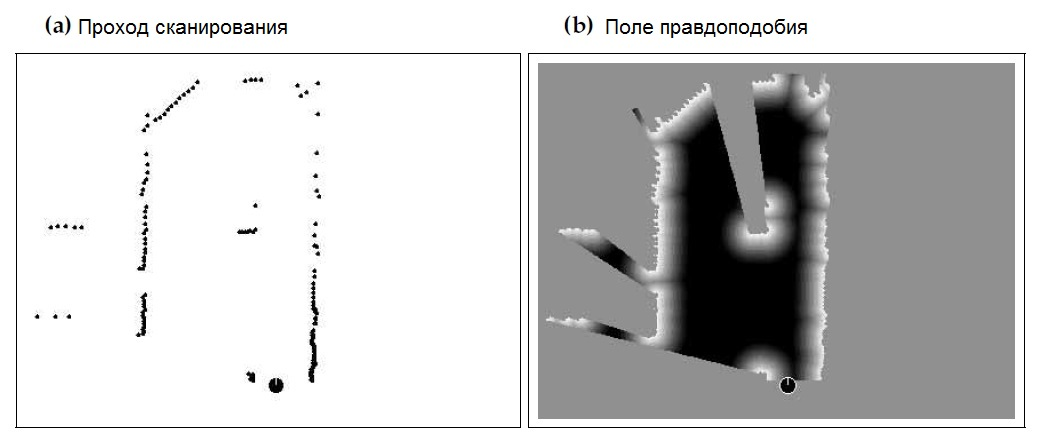
\includegraphics[width=0.85\linewidth]{611orig}}
	\caption{ (  Рис. 6.11 (a) Проход сканирования при виде сверху. Робот расположен в нижней части чертежа, и выполняет сканирование близлежащей области в 180 точках впереди робота. (b) На основе прохода сканирования генерируется функция правдоподобия. Чем темнее область, тем меньше правдоподобие обнаружения объекта в этой точке. Обратим внимание, что занятые области белые, поэтому штраф не накладывается.)}
	\label{fig:611orig}
\end{figure}

Поля правдоподобия по выделенному пространству могут также определяться для последнего прохода, который, фактически, и определяет карту. На Рис 6.11 показано такое поле правдоподобия. Оно играет важную роль в методах совмещениях отдельных проходов сканирования. \\

\textbf{6.5 Модели измерений на основе корреляции} \\

В литературе описаны несколько моделей датчиков расстояния, измеряющих корреляцию между измерением и картой.\\
НАЛОЖЕНИЕ КАРТ\\ Популярный метод
называется \textit{наложением карт}. Наложение карт требует методов, которые будут описаны позже, в частности, возможности превращать данные проходов сканирования в карты занятости. Обычно, при наложении карт небольшое число последовательных проходов сканирования преобразуются в локальные карты, обозначаемые $m_{local}$. На Рис. 6.12 показана такая локальная карта, здесь в виде карты сетки занятости. В модели измерения датчика сравниваются \textit{локальная карта} $m_{local}$ и глобальная карта $m$. Чем более схожи $m$ и $m_{local}$, тем больше $p(m_{local} | x_t, m)$. Поскольку локальная карта отображается относительно положения робота, это сравнение требует преобразования ячеек локальной карты в координатную сетку глобальной карты. 
Такое преобразование может быть выполнено аналогично выражению преобразования координат (6.32), выполненное для измерений датчиков, используемых в модели поля правдоподобия. Если робот находится в положении $x_t$, определим  ячейку сетки на локальной карте, соответствующую глобальным координатам $(x\,y)^T$, как $m_{x,y,local}(x_t)$. 

\begin{figure}[H]
	\center{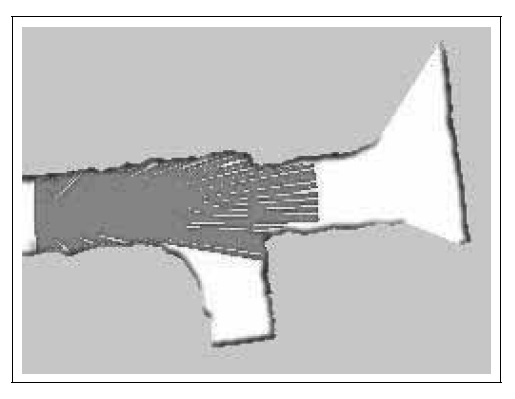
\includegraphics[width=0.8\linewidth]{612orig}}
	\caption{ (  Рис. 6.12 Пример локальной карты, сгенерированной из 10 измерений расстояния, из которых показано одно.)}
	\label{fig:612orig}
\end{figure}

Как только обе карты приведены к эталонной системе отсчёта, их можно сравнить с помощью функции корреляции карты, определённой следующим образом:\\

(6.35)
$$\rho_{m,m_{local},x_t}=\frac{\sum_{x,y}(m_{x,y}-\bar{m})\cdot(m_{x,y,local}(x_t)-\bar{m})}{\sqrt{\sum_{x,y}(m_{x,y}-\bar{m})^2\sum_{x,y}(m_{x,y,local}(x_t)-\bar{m})^2}}$$

Здесь сумма оценивается для всех ячеек, определённых на обеих картах, а $\bar{m}$ означает среднее значение по картам:\\

(6.36)
$$\bar{m}=\frac{1}{2N}\sum_{x,y}(m_{x,y}+m_{x,y,local})$$

Здесь $N$ определяет количество перекрывающихся элементов между локальной и глобальной картами.  Масштаб корреляции $\rho_{m,m_{local},x_t}$ меняется в диапазоне  $\pm1$. Наложение карт интерпретирует значение\\

(6.37)
$$p(m_{local}|x_t,m)=\max\{\rho_{m,m_{local},x_t},0\}$$

как вероятность локальной карты, наложенная на глобальную карту $m$ и положение робота $x_t$. Если локальная карта сгенерирована из одиночного сканирования расстояния $z_t$, эта вероятность заменяет вероятность измерения $p(z_t | x_t, m)$.

Наложение карт имеет ряд особенностей. Аналогично модели поля правдоподобия, его легко вычислить, хотя, в результате, не получается гладких распределений вероятности параметра положения $x_t$. Одним из способов приблизительно оценить поле правдоподобия (и достичь гладкости) является свёртка карты $m$ гауссовым ядром сглаживания, и выполнение наложения карт для уже сглаженной карты.

Ключевым преимуществом наложения карт над полями правдоподобия является явный учёт свободного пространства в сравнении двух карт. Метод поля правдоподобия учитывает только конечную точку сканирования, которая, по определению, соответствует занятому пространству (или шумам). С другой стороны, многие методы строят локальных карт за пределами досягаемости датчиков. Например, многие методы строят круговые карты вокруг робота, устанавливая значение вероятности 0,5 для зоны за пределами измерений датчиков. В таких случаях имеется опасность, что в результате наложения карт будут учтены зоны за пределами текущего радиуса измерений, как если бы датчик «видел сквозь стены». Такие побочные эффекты присутствуют в некоторых реализациях наложения карт.

Ещё одним недостатком наложения карт является отсутствие внятного физического обоснования. Корреляции представляют собой нормализованное квадратичное расстояние между объектами карт, а не шумовые характеристики датчиков расстояния.\\

\textbf{6.6 Модели измерений на основе признаков} \\

\textbf{6.6.1 Извлечение признаков}\\

Все модели датчиков, обсуждаемые до текущего момента, основаны на исходных измерениях.\\
ПРИЗНАКИ\\
Альтернативным подходом является извлечение признаков из измерений. 
Если определить механизм извлечения признаков в виде функции $f$, признаки, извлечённые из измерения расстояния, будут заданы как $f(z_t)$. Большинство выделителей признаков извлекают лишь небольшое количество признаков из измерений датчика высокой размерности. Главным преимуществом такого подхода является колоссальное уменьшение вычислительной сложности. Выполнение оценок в пространстве состояний высокой размерности может оказаться весьма затратным, и подобные операции в пространстве признаков с малой размерностью на порядки эффективнее. 

Обсуждение отдельных алгоритмов извлечения признаков не входит в область описания книги. В литературе предложен широкий набор признаков для самых различных датчиков. Для датчиков расстояния обычно определяют линии, углы или локальные минимумы сканирования расстояния, соответствующие стенам, углам или объектам, таким, как стволы деревьев. Использование камер для навигации относится к области компьютерного зрения, развитие которой породило множество методов извлечения признаков из изображений с камеры. Популярные признаки для изображений включают грани, углы, контрастные узоры и другие чётко различимые элементы. В робототехнике в качестве признаков часто применяются местоположения, например, проходы и пересечения.\\

\textbf{6.6.2 Измерения на основе ориентиров} \\

Во многих областях робототехники признаки соответствуют чётко различимым объектам физического мира. Например, в замкнутых помещениях признаками могут быть дверные косяки, подоконники, а на открытом пространстве – стволы деревьев или углы зданий.\\  
ОРИЕНТИРЫ \\
В робототехнике принято называть такие физические объекты \textit{ориентирами}, чтобы показать, что они используются для навигации робота.

Наиболее распространённая модель для обработки ориентиров подразумевает, что датчик способен измерить расстояние и направление на ориентир относительно локальной координаты системы робота.\\ 
ДАТЧИК РАССТОЯНИЯ И НАПРАВЛЕНИЯ\\
Такие датчики называются \textit{датчиками расстояния и направления}. Наличие таких датчиков не является неправдоподобным допущением, поскольку любой локальный признак, извлечённый из сканирования расстояния, содержит информацию о расстоянии и направлении, а также и о визуальных признаках, полученных со стереокамеры.\\
СИГНАТУРА ОРИЕНТИРА\\ Кроме этого, выделитель признаков может генерировать \textit{сигнатуру}. В  рамках изложения в книге будем считать сигнатурой числовое значение (например, среднее значение цвета). Это может быть и целое число, характеризующее тип ориентира, и многомерный вектор, характеризующий, скажем, его высоту и цвет.

Если определить расстояние как $r$, ориентацию как $\phi$, а сигнатуру $s$, вектор признаков задан коллекцией триплетов\\

(6.38)
\begin{minipage}{0.2\textwidth}
	\begin{equation*}
	f(z_t)=\{f_t^1,f_t^2,...\}=\{	\left(\begin{array}{c}
	r_t^1\\
	\phi_t^1\\
	s_t^1\\
	\end{array}\right)
	,
	\left(\begin{array}{c}
	r_t^2\\
	\phi_t^2\\
	s_t^2\\
	\end{array}\right)
	,...\}
	\end{equation*}
\end{minipage}\\

Количество признаков, идентифицированных на каждом такте времени, различается. Но множество вероятностных алгоритмов подразумевает условную независимость между признаками \\

(6.39)
$$p(f(z_t)|x_t,m)=\prod_i p(t_t^i,\phi_t^i,s_t^i|x_t,m)$$

Условная независимость применима, если шум каждого отдельного измерения $(r_t^i\, \phi^i_t\, s^i_t)^T$ не зависит от шума других измерений $(r_t^i\, \phi^i_t\, s^i_t)^T$ (для $i \neq j$). При допущении условной вероятности в один момент времени возможно обработать только один признак, также, как было сделано в нескольких моделях измерения расстояния. Это значительно облегчает разработку алгоритмов, реализующих вероятностные модели измерений. 

Начнём с определения модели датчика для признаков. В начале главы было выделено два типа карт: \textit{карты на основе признаков} и \textit{карты на основе местоположения}. Модели измерения на основе ориентиров обычно определены только для карт на основе признаков. Читатель может припомнить, что такие карты состоят из списков признаков $m = \{m_1, m_2, . . .\}$, каждый из которых может иметь сигнатуру и \textit{координату местоположения}. Местоположение признака, обозначенное $m_{i,x}$ и $m_{i,y}$, обозначает просто координаты на глобальной координатной сетке карты.

Вектор измерения для датчика ориентиров без учёта шума легко определить, используя обычные геометрические зависимости. Смоделируем шумы при восприятии ориентиров с помощью независимого гауссового шума по расстоянию, направлению и сигнатуре. Результирующая модель измерений сформулирована для случая, когда $i$-ый признак в момент времени $t$ соответствует $j$-му ориентиру на карте. Как обычно, положение робота задано в виде $x_t = (x\,y\,\theta)^T$ .\\

(6.40)
\begin{minipage}{0.2\textwidth}
	\begin{equation*}
	\left(\begin{array}{c}
	r_t^i\\
	\phi_t^i\\
	s_t^i\\
	\end{array}\right)
	=
	\left(\begin{array}{c}
	\sqrt{(m_{j,x}-x)^2+(m_{j,y}-y)^2}\\
	\text{atan}2(m_{j,y}-y,m_{j,x}-x)-\theta\\
	s_j\\
	\end{array}\right)
	+
	\left(\begin{array}{c}
	\varepsilon_{\sigma_r^2}\\
	\varepsilon_{\sigma_\phi^2}\\
	\varepsilon_{\sigma_s^2}\\
	\end{array}\right)
	\end{equation*}
\end{minipage}\\

Здесь $\varepsilon_{\sigma_r}$, $\varepsilon_{\sigma_\phi}$, и $\varepsilon_{\sigma_s}$ - переменные ошибки в виде гауссовых функций с нулевым математическим ожиданием и стандартными отклонениями $\sigma_r$, $\sigma_\phi$, и $\sigma_s$, соответственно.\\

\textbf{6.6.3 Модель датчика с известным соответствием}\\

ПРОБЛЕМА АССОЦИАЦИИ ДАННЫХ\\
Одна из главных проблем датчиков расстояния/направления известна как \textit{проблема ассоциации данных}. Она возникает, когда невозможно различить ориентиры, и появляется некоторая остаточная неопределённость по отношению к идентификации ориентира.\\ ПЕРЕМЕННАЯ СООТВЕТСТВИЯ\\ Для разработки модели датчика расстояния/направления будет полезно ввести переменную соответствия между признаком $f_t^i$ и ориентиром $m_j$ на карте. Эта переменная будет определена как $c^i_t$ с $c^i_t\in\{1, . . . , N + 1\}$.
$N$ – количество ориентиров на карте $m$. Если $c^i_t = j\leq N$, тогда $i$-ый признак, наблюдаемый в момент времени $t$, соответствует $j$-ому ориентиру на карте. Другими словами, $c^i_t$ - истинный идентификатор наблюдаемого признака. Единственное исключение происходит при $c^i_t = N + 1$: В данном случае наблюдение признака не соответствует ни одному признаку карты $m$. Этот случай важен для обработки фантомных ориентиров, а также очень актуален для составления карт в робототехнике, когда робот может столкнуться с прежде неизвестными ориентирами.   

В Таблице 6.4 показан алгоритм вычисления вероятности  признака
$f_t^i$ с известным соответствием $c^i_t\leq N$. В строках 3 и 4 вычисляются верные расстояние и направление на ориентир. Вероятность для измеренных расстояния и направления вычисляются в строке 5, где подразумевая независимость шумов.
Как читатель может легко убедиться, алгоритм реализует уравнение (6.40).

\begin{table}[H]
\begin{center}
\begin{tabular}{|l|}
\hline
{}\\
1: \hspace{3mm} Algorithm landmark\_model\_known\_correspondence $(f_t^i,c_t^i,x_t,m):$ \\
{}\\
2:\hspace{7mm}$j=c_t^i$\\
3:\hspace{7mm}$\hat{r}=\sqrt{(m_{j,x}-x)^2+(m_{j,y}-y)^2}$\\
4:\hspace{7mm}$\hat{\phi}=\text{atan}2(m_{j,y}-y,m_{j,x}-x)$\\
5:\hspace{7mm}$q=\text{\textbf{prob}}(r_t^i-\hat{r},\sigma_r)\cdot\text{\textbf{prob}}(\phi_t^i-\hat{\phi},\sigma_\phi)\cdot\text{\textbf{prob}}(s_t^i-s_j,\sigma_s)$\\
6:\hspace{7mm}$\textit{return}\,q$\\
{}\\
\hline
\end{tabular}
\caption{(Таблица 6.4 Алгоритм вычисления правдоподобности измерения ориентира. Алгоритм требует на вход наблюдаемый ориентир $f_t^i = (r_t^i\,\phi^i_t\, s^i_t)^T$, истинное обозначение признака $c^i_t$, положение робота $x_t = (x\,y\,\theta)^T$, и карта $m$. На выходе вычисляется численное значение вероятности $p(f_t^i | c^i_t, m, x_t)$. )}
\end{center}
\end{table}

\textbf{6.6.4 Определение положения на основе выборки}\\

Иногда желательно сделать выборку местоположений робота $x_t$, соответствующую измерению $f_t^i$ с признаком $c^i_t$. Мы уже сталкивались с такими алгоритмами выборки в прошлой главе, при обсуждении модели движения робота. Такие модели выборки также применимы для моделей датчиков. Например, при глобальной локализации робота будет полезным сгенерировать такую выборку положений робота, которая будет включать измерения датчиков для генерации начальных гипотез локализации. 

Хотя, в общем случае, выборка положений  $x_t$, соответствующая измерению датчика $z_t$, затруднена, для нашей модели ориентиров возможно предложить эффективный алгоритм выборки, хотя и с некоторыми допущениями. В частности, необходимо знать априорную вероятность $p(x_t |c^i_t, m)$. Для простоты, допустим, что эта априорная вероятность равномерна (в общем случае это не так!).
Тогда, согласно теореме Байеса\\

(6.41)
\begin{equation*}
\begin{split}
p(x_t|f_t^i,c_t^i,m)&=\eta\,p(f_t^i|c_t^i,x_t,m)\,p(x_t|c_t^i,m)\\
&=\eta\,p(f_t^i|c_t^i,x_t,m)
\end{split}
\end{equation*}

Выборка из $p(x_t | f_t^i, c^i_t, m)$ теперь может быть выполнена из  «обратной» модели датчика $p(f_t^i | c^i_t, x_t, m)$. В Таблице 6.5 приводится алгоритм, выполняющий выборку положений $x_t$. Правда, такая выборка имеет особенность: даже в случае отсутствия шума, наблюдение ориентира не определяет точного положения робота. Согласно алгоритму, робот может находиться в произвольной точке окружности вокруг ориентира, диаметр которой равен расстоянию до ориентира. Неопределённость положения робота следует также из факта того, что параметры расстояния и направления накладывают два ограничения в трехмерном пространстве положений робота.

\begin{table}[H]
\begin{center}
\begin{tabular}{|l|}
\hline
{}\\
1: \hspace{3mm} Algorithm sample\_landmark\_model\_known\_correspondence $(f_t^i,c_t^i,m):$ \\
{}\\
2:\hspace{7mm}$j=c_t^i$\\
3:\hspace{7mm}$\hat{\gamma}=\text{rand}(0,2\pi)$\\
4:\hspace{7mm}$\hat{r}=r_t^i+\text{sample}(\sigma_r)$\\
5:\hspace{7mm}$\hat{\phi}=\phi_t^i+\text{sample}(\sigma_\phi)$\\
6:\hspace{7mm}$x=m_{j,x}+\hat{r}\cos\hat{\gamma}$\\
7:\hspace{7mm}$y=m_{j,y}+\hat{r}\sin\hat{\gamma}$\\
8:\hspace{7mm}$\theta=\hat{\gamma}-\pi-\hat{\phi}$\\
9:\hspace{7mm}$\textit{return}\,(x\,y\,\theta)^T$\\
{}\\
\hline
\end{tabular}
\caption{(Таблица 6.5 Алгоритм выполнения выборки положений из измерения ориентира $f_t^i = (r_t^i\, \phi^i_t\, s^i_t)^T$ с известным обозначением  $c^i_t$.)}
\end{center}
\end{table}

Для реализации алгоритма выборки, необходимо выполнить выборку оставшегося свободного параметра, определяющего конкретное место окружности, в котором и находится робот. Этот параметр называется $\hat{\gamma}$ в Таблице 6.5, и выбирается случайным образом в строке 3. В строках 4 и 5 происходит изменение измеренных расстояния и направления с использованием факта симметричного отображения математического ожидания и измерения в виде нормального распределения. Наконец, в строках с 6 по 8 восстанавливается положение, соответствующее $\hat{\gamma}$, $\hat{r}$, и $\hat{\phi}$.

На Рис. 6.13 показано распределение положений $p(x_t | f_t^i, c^i_t, m)$ (левая схема)  и выборки, выполненной алгоритмом \textbf{sample\_landmark\_model\_known\_correspondence} (правая схема). Апостериорное распределение проектируется на плоскость в виде кольца вокруг измеренного расстояния $r_t^i$. В трехмерном пространстве положений образуется спираль, которая разворачивается из кольца с углом $\theta$.\\

\textbf{6.6.5 Дальнейшие соображения}\\

В обоих алгоритмах измерений на основе ориентиров подразумевается, что соответствие известно. Случай, когда соответствие неизвестно, будет детально описан в следующих главах при обсуждении алгоритмов локализации и построения карт. 

\begin{figure}[H]
	\center{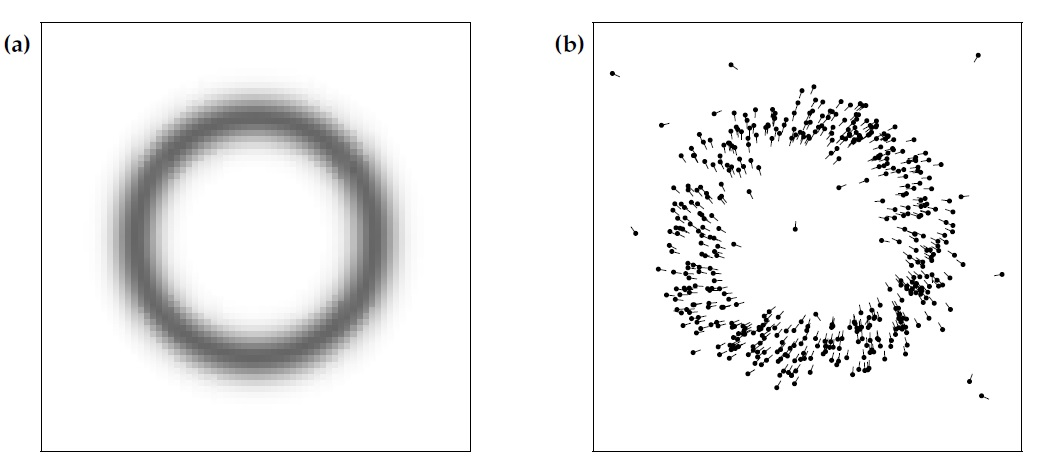
\includegraphics[width=0.9\linewidth]{613orig}}
	\caption{ (  Рис. 6.13 Модель обнаружения ориентира: (a) Согласно апостериорному распределению положения робота, был обнаружен ориентир на расстоянии 5 м и под относительным углом направления 30 градусов (в проекции на плоскость). (b) Выборка положений робота, сгенерированная на основании обнаружения. Линиями обозначена ориентация положений по углу направления.)}
	\label{fig:613orig}
\end{figure}

Следует добавить несколько слов о сигнатуре ориентира. В большинстве опубликованных алгоритмов черты внешнего вида в явном виде не используются. Если сигнатура не учитывается, все ориентиры выглядят одинаково, и проблема ассоциации данных при оценке переменной соответствия усугубляется. Мы включили в модель сигнатуру потому, что это значимый источник информации, которую часто можно легко извлечь из показаний датчиков. 

Как отмечено выше, основной причиной использования признаков вместо полного вектора измерений является экономия вычислительных ресурсов. Гораздо проще обрабатывать несколько сот признаков, чем несколько миллионов измерений расстояния. Представленная здесь модель крайне груба и, определённо, не отражает каких-либо физических законов, лежащих в основе процесса измерений датчика. Несмотря на это, способна хорошо работать в большом количестве прикладных задач. 

Важно заметить, что операция преобразование измерений в признаки также имеет свою цену.\\ ДОСТАТОЧНЫЕ СТАТИСТИКИ\\
В литературе по робототехнике признаки часто (ошибочно) воспринимаются, как \textit{достаточные статистики} вектора измерений $z_t$. Пусть $X$ будет интересующей переменной (например, картой, положением, и т. д.), а $Y$ – какой-либо другой информацией, которую хотелось бы учитывать (скажем, прошлые измерения датчиков). Тогда $f$ будет достаточной статистикой $z_t$ при условии\\

(6.42)
$$p(X|z_t,Y)+p(X|f(z_t),Y)$$

На практике большое количество информации просто утрачивается в силу использования признаков вместо полного вектора измерений. Эта утраченная информация усугубляет некоторые проблемы, например, проблему ассоциации данных при определении, не оказался ли робот в ранее посещённом местоположении. Проблему извлечения признаков легко понять умозрительно: Если открыть глаза, визуальная картина окружающего, скорее всего, окажется достаточной, чтобы недвусмысленно определить местоположение, даже если до этого момента присутствовала общая неопределённость. Если же, с другой стороны, воспринимать только отдельные признаки, например, относительное расположение дверных косяков и подоконников, скорее всего, степень уверенности будет значительно ниже и получаемой информации будет недостаточно для выполнения глобальной локализации. 

С появлением всё более быстрых компьютеров признаки в области робототехники постепенно теряют значимость, особенно при использовании датчиков расстояния. Многие новейшие алгоритмы полагаются на плотные векторы измерений и используют столь же плотные карты на основе местоположений для отображения окружающего пространства. Тем не менее, признаки хорошо подходят для использования в образовательных целях. Они позволяют представить базовые концепции вероятностной робототехники и, при правильном подходе к задачам, например, задаче соответствия, могут быть использованы даже для случаев, когда карты состоят из плотных наборов точек сканирования. В силу этого, часть алгоритмов, представленных в книге, сначала описываются в представлении признаков, а затем обобщаются для использования исходных измерений датчиков.\\

\textbf{6.7 Практические соображения}\\

В этом разделе описан ряд моделей измерения. Большое внимание было уделено моделям датчиков расстояния в силу их большой значимости для робототехники. Однако, описанные модели представляют только иллюстрацию для значительно более широкого класса вероятностного моделирования. При выборе верной модели важно найти правильное сочетание физического реализма и наиболее значимых свойств алгоритма на её основе. Например, было замечено, что физически реалистичная модель датчика расстояния может выдавать негладкие вероятности при определении положения робота, и это может стать проблемой для алгоритмов, скажем, многочастичных фильтров. Поэтому, физический реализм не является единственным критерием выбора модели датчика. Столь же важно учитывать применимость модели для алгоритма, в котором она применяется. 

В большинстве случаев, чем точнее модель, тем лучше. Например, чем больше информации удаётся извлечь из показаний датчика, тем лучше. Модели на основе признаков извлекают сравнительно мало информации в силу того, что выделитель признаков проектирует показания датчиков с высокой размерностью в пространство с более низкой размерностью. В результате, методы на основе признаков демонстрируют худшие результаты, что, отчасти, компенсируется их большей вычислительной эффективностью. 

При настройке внутренних параметров модели измерений часто полезно искусственно увеличить неопределённость в силу наличия основного ограничения вероятностного подхода: чтобы сделать вероятностные методы вычислительно разрешимыми, приходится игнорировать существующие в физическом мире зависимости и огромное множество переменных, которые эти зависимости образуют. Если такие зависимости не моделировать, алгоритмы, собирающие данные на малом количестве измерений, часто становятся чрезмерно «самоуверенными».\\
САМОУВЕРЕННОСТЬ\\ Такая
\textit{самоуверенность}, в итоге, приводит к неверным заключениям, что негативно сказывается на результатах. На практике часто хорошей идеей является уменьшение количества информации, получаемой из показаний датчика. Проектирование измерения в пространство признаков с низкой размерностью – это лишь один способ выполнить такое уменьшение, который, вдобавок, подвержен описанным выше ограничениям. Равномерное экспоненциальное разложение информации в модели измерений с параметром $\alpha$, как обсуждалось в разделе 6.3.4, значительно лучше, поскольку не увеличивает дисперсию на выходе вероятностного алгоритма.\\

\textbf{6.8 Выводы}\\

В этом разделе описаны вероятностные модели измерений.\\

• Начиная с моделей датчиков расстояния, в частности, лазерных, были описаны модели измерений $p(z_t^k | x_t, m)$. В первой модели для определения формы распределения $p(z_t^k | x_t, m)$ на основе известных картах $m$ и положений  $x_t$ было использовано бросание лучей. Была определена модель смеси, учитывающая различные виды шумов, которые могут повлиять на измерения расстояния.\\ 

• Был описан метод максимального правдоподобия для определения внутренних параметров шума модели измерений. Поскольку модель измерения представлена методом смешения, была предложена итерационная процедура оценки максимального правдоподобия. Предложенный подход является экземпляром алгоритма максимизации ожидания, который изменяет такт вычисления ожидания в соответствии с типом ошибки измерения и тактом максимизации, который в закрытом виде находит наилучший набор внутренних параметров для этих ожиданий. \\

• Альтернативная модель измерений для датчиков расстояния основана на полях правдоподобия. В этом методе для моделирования вероятности $p(z_t^k | x_t, m)$ используется ближайшее расстояние в двухмерных координатах. Заметим, что такой подход даёт более гладкие распределения $p(z_t^k | x_t, m)$, но это происходит за счёт появления некоторых нежелательных побочных эффектов.Так, в методе полей правдоподобия игнорируется информацию относительно свободного пространства и не учитываются противоречия интерпретации измерений расстояния.\\

• Третья модель измерения основана на наложении карт. При наложении карт происходит наложение проходов сканирования датчика на локальные карты в целях корреляции их с глобальными. Такой подход недостаточно физически обоснован, зато может быть очень эффективно реализован на практике. \\

• Обсуждалось, каким образом предварительные вычисления могут уменьшить вычислительную эффективность в задачах реальном времени. В модели измерения на основе лучей предварительные вычисления выполняются в 3D, а поля правдоподобия требуют предварительных расчётов в 2D.\\

• Была представлена модель датчика на основе признаков, в которой робот выполняет извлечение данные о расстоянии, угле направления и сигнатуре близлежащих ориентиров. Методы на основе признаков извлекают признаки из исходных измерений датчиков, уменьшая  размерность измерений датчиков на несколько порядков. \\

• В конце главы в ходе дискуссии о практических аспектах были выявлены некоторые трудности, которые могут возникнуть в конкретных реализациях. \\

\textbf{6.9 Библиографические примечания}\\

В этой главе приводятся лишь единичные примеры обширной литературы по физическому моделированию датчиков. Более точные модели сонаров можно найти в работах Блахата (Blahut et al., 1991), Грунбаума (Grunbaum et al., 1992) и Эттера (Etter, 1996). Модели лазерных датчиков расстояния были описаны Рисом (Rees, 2001). Эмпирическое обсуждение адекватных моделей шумов было проведено Сахиным (Sahin et al., 1998). В сравнении с этими моделями, обсуждаемые в книге модели весьма грубы.

Ранние разработки моделей на основе лучей для дальномеров можно найти в основополагающей работе Моравица (Moravec, 1988). Похожая модель была позже использована в локализации мобильного робота Бургардом (Burgard et al., 1996). Модель на основе лучей наподобие описанной, вместе с предварительным вычислением измерений расстояния была впервые описана Фоксом (Fox et al.,1999b). Поля правдоподобия впервые были опубликованы в работе Труна (Thrun, 2001), хотя они тесно связаны с обширной литературой по методам наложения сканирования (Besl and McKay 1992). Фактически, их можно считать мягким вариантом модели корреляции, описанной Конолигом и Чау (Konolige and Chou, 1999). Методы вычисления корреляции между картами сеток занятости также стали довольно популярными. Трун (Thrun, 1993) вычислил сумму квадратичной ошибки между отдельными ячейками двух карт сетей. Шили и Краули (Schiele and Crowley, 1994) представили сравнение разных моделей, включая методы на основе корреляции. Ямагучи и Ленгли (Yamauchi and Langley, 1997) проанализировали надёжность наложения карт в динамических средах. Дакит и Немцоу (Duckett and Nehmzow, 2001) преобразовали локальные сети занятости в гистограммы, которые можно сравнивать между собой более эффективно. 

Измерения расстояния и угла направления для нахождения ориентиров общеприняты в литературе по SLAM. Возможно, впервые они были упомянуты Леонардом и Дюран-Уайтом (Leonard and Durrant-Whyte, 1991). В более ранней работе Краули (Crowley, 1989) вывел модели измерения для прямолинейных объектов.\\

\textbf{6.10 Упражнения}\\

1. Многие ранние образцы роботов выполняли навигацию, используя признаки на основе искусственных ориентиров, помещённые в среду так, чтобы их было легко различить. Хорошим местом для размещения таких маркеров был потолок (а почему?). Классический пример визуального маркера: допустим, на потолке закреплён  маркер следующего вида:

\begin{figure}[H]
	\center{
\includegraphics[width=0.2\linewidth]{614orig}}
	\label{fig:614orig}
\end{figure}

Пусть глобальные координаты маркера будут $x_m$ и $y_m$, а ориентация в глобальной системе координат $\theta_m$. Определим положение робота через $x_r$, $y_r$, и $\theta_r$.\\

Теперь допустим, что был определён маршрут, в ходе которого маркер может быть обнаружен на плоскости изображения перспективной камеры. Пусть $x_i$ и $y_i$ определяют координаты маркера на плоскости изображения, а $\theta_i$ – угол направления.
Камера имеет фокусное расстояние $f$. С точки зрения проективной геометрии известно, что каждое смещение $d$ в пространстве $x-y$ проектируется в виде пропорционального смещения $d\cdot\frac{f}{h}$ на плоскости изображения. (Необходимо сделать некоторые допущения относительно выбранной системы координат и выполнить их в явном виде).\\

Вопросы:\\

(a) Математически описать ожидаемое местоположение маркера (в глобальных координатах $x_m$, $y_m$, $\theta_m$), при известных координатах изображения $x_i$, $y_i$, $,\theta_i$  и положении робота в $x_r$, $y_r$, $\theta_r$.\\

(b) Привести математическое выражение для вычисления координат изображения $x_i$, $y_i$, $\theta_i$ на основе положения робота $x_r$, $y_r$, $\theta_r$ и координат маркера $x_m$, $y_m$, $\theta_m$.\\

(c) Привести математическое выражение для определения координат робота $x_r$, $y_r$, $\theta_r$, допуская, что известны истинные координаты маркера $x_m$, $y_m$, $\theta_m$, а координаты изображения $x_i$, $y_i$, $\theta_i$.\\

(d) Пока подразумевалось, что маркер только один. Теперь допустим, что имеется несколько неразличимых между собой маркеров, как показанный выше. 
Сколько таких маркеров должен воспринимать робот, чтобы надёжно определить положение? Нарисовать такую конфигурацию и объяснить, почему она достаточна.\\ 

Подсказка: Нет необходимости учитывать неопределённость измерения для ответа на этот вопрос. Также, обратите внимание, что маркер симметричен, поскольку  для ответа на вопрос это имеет значение! \\

2. В этом упражнении требуется обобщить вычисление из прошлого упражнения, чтобы учесть ошибки ковариации. Для упрощения вычислений допустим, что маркер несимметричен и можно оценить его абсолютный угол поворота :

\begin{figure}[H]
	\center{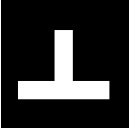
\includegraphics[width=0.2\linewidth]{615orig}}
	\label{fig:615orig}
\end{figure}

Также, для простоты допустим, что значение угла поворота не содержит шумов, но оценки $x-y$ координат в плоскости изображения могут быть зашумлены. Определим, что измерения будут подвержены гауссовскому шуму с нулевым математическим ожиданием и ковариацией \\

\begin{minipage}{0.2\textwidth}
	\begin{equation*}
	\sum=
	\left(\begin{array}{ccc}
	\sigma^2&0&0\\
	0&\sigma^2&0\\
	0&0&0\\
	\end{array}\right)
	\end{equation*}
\end{minipage}\\

для некоторого положительного значения $\sigma^2$.\\

Вычислить соответствующую ковариацию для трёх предыдущих упражнений. В частности,\\

(a) Даны координаты изображения $x_i$, $y_i$, $\theta_i$ и координаты робота
$x_r$, $y_r$, $\theta_r$. Определить ковариацию ошибки для значений $x_m$, $y_m$, $\theta_i$.\\

(b) Даны координаты робота $x_r$, $y_r$, $\theta_r$ и ковариация маркера $x_m$, $y_m$, $\theta_m$. Определить ковариацию ошибки для значений $x_i$, $y_i$, $\theta_i$.\\

(c) Задана ковариация маркера $x_m$, $y_m$, $\theta_m$ и координаты изображения $x_i$, $y_i$, $\theta_i$. Определить ковариацию ошибки для значений $x_r$, $y_r$, $\theta_r$.\\

Обратите внимание, что не все эти распределения могут быть гауссовыми. Для этого упражнения допустимо применить разложение в ряд Тейлора для получения гауссового апостериорного распределения, но требуется объяснить, каким образом это нужно делать. \\

3. Необходимо реализовать алгоритм \textbf{sample\_marker\_model}, который принимает на вход положение маркера $x_m$, $y_m$, $\theta_m$ и местоположение найденного маркера на плоскости изображения $x_i$, $y_i$, $\theta_i$, и сгенерировать в виде выходных данных выборку положений робота $x_r$, $y_r$, $\theta_r$. Использовать симметричный маркер из упражнения 1:

\begin{figure}[H]
	\center{
\includegraphics[width=0.2\linewidth]{614orig}}
	\label{fig:614orig}
\end{figure}

Изобразить график выборки для координат робота $x_r$ и $y_r$ со следующими параметрами (для этого распределения можно игнорировать угол ориентации $\theta_r$ ).

\begin{table}[H]
\begin{center}
\begin{tabular}{|c|c|c|c|c|}
\hline
\text{problem \#}&\hspace{2mm}$x_m$\hspace{6mm}$y_m$\hspace{8mm}$\theta_m$ &\hspace{2mm}$x_i$\hspace{6mm}$y_i$\hspace{8mm}$\theta_i$&$h/f$&$\sigma^2$\\
\hline
\#1&\hspace{2mm}$0\text{см}$\hspace{6mm}$0\text{см}$\hspace{8mm}$0^\circ$&\hspace{2mm}$0\text{см}$\hspace{6mm}$0\text{см}$\hspace{8mm}$0^\circ$&$200$&$0.1\text{см}^2$\\
\hline
\#2&\hspace{2mm}$0\text{см}$\hspace{6mm}$0\text{см}$\hspace{8mm}$0^\circ$&\hspace{2mm}$1\text{см}$\hspace{6mm}$0\text{см}$\hspace{8mm}$0^\circ$&$200$&$0.1\text{см}^2$\\
\hline
\#3&\hspace{2mm}$0\text{см}$\hspace{6mm}$0\text{см}$\hspace{8mm}$0^\circ$&\hspace{2mm}$2\text{см}$\hspace{6mm}$0\text{см}$\hspace{8mm}$45^\circ$&$200$&$0.1\text{см}^2$\\
\hline
\#4&\hspace{2mm}$0\text{см}$\hspace{6mm}$0\text{см}$\hspace{8mm}$0^\circ$&\hspace{2mm}$2\text{см}$\hspace{6mm}$0\text{см}$\hspace{8mm}$45^\circ$&$200$&$1.0\text{см}^2$\\
\hline
\#5&\hspace{3mm}$50\text{см}$\hspace{6mm}$150\text{см}$\hspace{5mm}$10^\circ$&\hspace{2mm}$1\text{см}$\hspace{6mm}$6\text{см}$\hspace{8mm}$200^\circ$&$250$&$0.5\text{см}^2$\\
\hline
\end{tabular}
\end{center}
\end{table}

На всех графиках следует изобразить координатные оси с единицами измерения. Примечание: если не сможете предложить алгоритм в точном виде, предложить приближенный алгоритм и объяснить соображения приближения. \\

4. Для этого упражнения понадобится доступ к любому роботу для работы внутри помещений, оснащённому сонаром. Разместить датчик перед плоской стеной, на расстоянии $d$ и под углом $\phi$. Подобрать и измерить частоту, при которой датчик обнаруживает стену. Отобразить значения расстояния $d$ на графике с шагом 0,5 м и углов $\phi$ с шагом 5 градусов. Что получилось в результате?




\end{document}